\documentclass[a4paper, 12pt]{article}
\usepackage[left=2cm,right=2cm, top=2cm,bottom=2cm,bindingoffset=0cm]{geometry}
\usepackage{cmap, amssymb, amsmath, amsthm, mathtools, mathtext}
\setcounter{MaxMatrixCols}{11}
\usepackage{upgreek}
\usepackage{setspace}
\usepackage[normalem]{ulem}

    \usepackage[breakable]{tcolorbox}
    \usepackage{parskip} % Stop auto-indenting (to mimic markdown behaviour)
    

    % Basic figure setup, for now with no caption control since it's done
    % automatically by Pandoc (which extracts ![](path) syntax from Markdown).
    \usepackage{graphicx}
    % Keep aspect ratio if custom image width or height is specified
    \setkeys{Gin}{keepaspectratio}
    % Maintain compatibility with old templates. Remove in nbconvert 6.0
    \let\Oldincludegraphics\includegraphics
    % Ensure that by default, figures have no caption (until we provide a
    % proper Figure object with a Caption API and a way to capture that
    % in the conversion process - todo).
    \usepackage{caption}
    \DeclareCaptionFormat{nocaption}{}
    \captionsetup{format=nocaption,aboveskip=0pt,belowskip=0pt}

    \usepackage{float}
    \floatplacement{figure}{H} % forces figures to be placed at the correct location
    \usepackage{xcolor} % Allow colors to be defined
    \usepackage{enumerate} % Needed for markdown enumerations to work
    \usepackage{geometry} % Used to adjust the document margins
    \usepackage{amsmath} % Equations
    \usepackage{amssymb} % Equations
    \usepackage{textcomp} % defines textquotesingle
    % Hack from http://tex.stackexchange.com/a/47451/13684:
    \AtBeginDocument{%
        \def\PYZsq{\textquotesingle}% Upright quotes in Pygmentized code
    }
    \usepackage{upquote} % Upright quotes for verbatim code
    \usepackage{eurosym} % defines \euro

    \usepackage{iftex}
    \ifPDFTeX
        \usepackage[T2A]{fontenc}
        \IfFileExists{alphabeta.sty}{
              \usepackage{alphabeta}
          }{
              \usepackage[mathletters]{ucs}
              \usepackage[utf8]{inputenc}
          }
    \else
        \usepackage{fontspec}
        \usepackage{unicode-math}
    \fi

    \usepackage{fancyvrb} % verbatim replacement that allows latex
    \usepackage{grffile} % extends the file name processing of package graphics
                         % to support a larger range
    \makeatletter % fix for old versions of grffile with XeLaTeX
    \@ifpackagelater{grffile}{2019/11/01}
    {
      % Do nothing on new versions
    }
    {
      \def\Gread@@xetex#1{%
        \IfFileExists{"\Gin@base".bb}%
        {\Gread@eps{\Gin@base.bb}}%
        {\Gread@@xetex@aux#1}%
      }
    }
    \makeatother
    \usepackage[Export]{adjustbox} % Used to constrain images to a maximum size
    \adjustboxset{max size={0.9\linewidth}{0.9\paperheight}}

    % The hyperref package gives us a pdf with properly built
    % internal navigation ('pdf bookmarks' for the table of contents,
    % internal cross-reference links, web links for URLs, etc.)
    \usepackage{hyperref}
    % The default LaTeX title has an obnoxious amount of whitespace. By default,
    % titling removes some of it. It also provides customization options.
    \usepackage{titling}
    \usepackage{longtable} % longtable support required by pandoc >1.10
    \usepackage{booktabs}  % table support for pandoc > 1.12.2
    \usepackage{array}     % table support for pandoc >= 2.11.3
    \usepackage{calc}      % table minipage width calculation for pandoc >= 2.11.1
    \usepackage[inline]{enumitem} % IRkernel/repr support (it uses the enumerate* environment)
    \usepackage[normalem]{ulem} % ulem is needed to support strikethroughs (\sout)
                                % normalem makes italics be italics, not underlines
    \usepackage{soul}      % strikethrough (\st) support for pandoc >= 3.0.0
    \usepackage{mathrsfs}
    

    
    % Colors for the hyperref package
    \definecolor{urlcolor}{rgb}{0,.145,.698}
    \definecolor{linkcolor}{rgb}{.71,0.21,0.01}
    \definecolor{citecolor}{rgb}{.12,.54,.11}

    % ANSI colors
    \definecolor{ansi-black}{HTML}{3E424D}
    \definecolor{ansi-black-intense}{HTML}{282C36}
    \definecolor{ansi-red}{HTML}{E75C58}
    \definecolor{ansi-red-intense}{HTML}{B22B31}
    \definecolor{ansi-green}{HTML}{00A250}
    \definecolor{ansi-green-intense}{HTML}{007427}
    \definecolor{ansi-yellow}{HTML}{DDB62B}
    \definecolor{ansi-yellow-intense}{HTML}{B27D12}
    \definecolor{ansi-blue}{HTML}{208FFB}
    \definecolor{ansi-blue-intense}{HTML}{0065CA}
    \definecolor{ansi-magenta}{HTML}{D160C4}
    \definecolor{ansi-magenta-intense}{HTML}{A03196}
    \definecolor{ansi-cyan}{HTML}{60C6C8}
    \definecolor{ansi-cyan-intense}{HTML}{258F8F}
    \definecolor{ansi-white}{HTML}{C5C1B4}
    \definecolor{ansi-white-intense}{HTML}{A1A6B2}
    \definecolor{ansi-default-inverse-fg}{HTML}{FFFFFF}
    \definecolor{ansi-default-inverse-bg}{HTML}{000000}

    % common color for the border for error outputs.
    \definecolor{outerrorbackground}{HTML}{FFDFDF}

    % commands and environments needed by pandoc snippets
    % extracted from the output of `pandoc -s`
    \providecommand{\tightlist}{%
      \setlength{\itemsep}{0pt}\setlength{\parskip}{0pt}}
    \DefineVerbatimEnvironment{Highlighting}{Verbatim}{commandchars=\\\{\}}
    % Add ',fontsize=\small' for more characters per line
    \newenvironment{Shaded}{}{}
    \newcommand{\KeywordTok}[1]{\textcolor[rgb]{0.00,0.44,0.13}{\textbf{{#1}}}}
    \newcommand{\DataTypeTok}[1]{\textcolor[rgb]{0.56,0.13,0.00}{{#1}}}
    \newcommand{\DecValTok}[1]{\textcolor[rgb]{0.25,0.63,0.44}{{#1}}}
    \newcommand{\BaseNTok}[1]{\textcolor[rgb]{0.25,0.63,0.44}{{#1}}}
    \newcommand{\FloatTok}[1]{\textcolor[rgb]{0.25,0.63,0.44}{{#1}}}
    \newcommand{\CharTok}[1]{\textcolor[rgb]{0.25,0.44,0.63}{{#1}}}
    \newcommand{\StringTok}[1]{\textcolor[rgb]{0.25,0.44,0.63}{{#1}}}
    \newcommand{\CommentTok}[1]{\textcolor[rgb]{0.38,0.63,0.69}{\textit{{#1}}}}
    \newcommand{\OtherTok}[1]{\textcolor[rgb]{0.00,0.44,0.13}{{#1}}}
    \newcommand{\AlertTok}[1]{\textcolor[rgb]{1.00,0.00,0.00}{\textbf{{#1}}}}
    \newcommand{\FunctionTok}[1]{\textcolor[rgb]{0.02,0.16,0.49}{{#1}}}
    \newcommand{\RegionMarkerTok}[1]{{#1}}
    \newcommand{\ErrorTok}[1]{\textcolor[rgb]{1.00,0.00,0.00}{\textbf{{#1}}}}
    \newcommand{\NormalTok}[1]{{#1}}

    % Additional commands for more recent versions of Pandoc
    \newcommand{\ConstantTok}[1]{\textcolor[rgb]{0.53,0.00,0.00}{{#1}}}
    \newcommand{\SpecialCharTok}[1]{\textcolor[rgb]{0.25,0.44,0.63}{{#1}}}
    \newcommand{\VerbatimStringTok}[1]{\textcolor[rgb]{0.25,0.44,0.63}{{#1}}}
    \newcommand{\SpecialStringTok}[1]{\textcolor[rgb]{0.73,0.40,0.53}{{#1}}}
    \newcommand{\ImportTok}[1]{{#1}}
    \newcommand{\DocumentationTok}[1]{\textcolor[rgb]{0.73,0.13,0.13}{\textit{{#1}}}}
    \newcommand{\AnnotationTok}[1]{\textcolor[rgb]{0.38,0.63,0.69}{\textbf{\textit{{#1}}}}}
    \newcommand{\CommentVarTok}[1]{\textcolor[rgb]{0.38,0.63,0.69}{\textbf{\textit{{#1}}}}}
    \newcommand{\VariableTok}[1]{\textcolor[rgb]{0.10,0.09,0.49}{{#1}}}
    \newcommand{\ControlFlowTok}[1]{\textcolor[rgb]{0.00,0.44,0.13}{\textbf{{#1}}}}
    \newcommand{\OperatorTok}[1]{\textcolor[rgb]{0.40,0.40,0.40}{{#1}}}
    \newcommand{\BuiltInTok}[1]{{#1}}
    \newcommand{\ExtensionTok}[1]{{#1}}
    \newcommand{\PreprocessorTok}[1]{\textcolor[rgb]{0.74,0.48,0.00}{{#1}}}
    \newcommand{\AttributeTok}[1]{\textcolor[rgb]{0.49,0.56,0.16}{{#1}}}
    \newcommand{\InformationTok}[1]{\textcolor[rgb]{0.38,0.63,0.69}{\textbf{\textit{{#1}}}}}
    \newcommand{\WarningTok}[1]{\textcolor[rgb]{0.38,0.63,0.69}{\textbf{\textit{{#1}}}}}


    % Define a nice break command that doesn't care if a line doesn't already
    % exist.
    \def\br{\hspace*{\fill} \\* }
    % Math Jax compatibility definitions
    \def\gt{>}
    \def\lt{<}
    \let\Oldtex\TeX
    \let\Oldlatex\LaTeX
    \renewcommand{\TeX}{\textrm{\Oldtex}}
    \renewcommand{\LaTeX}{\textrm{\Oldlatex}}
    % Document parameters
    % Document title
    \title{notebook}
    
    
    
    
    
    
    
% Pygments definitions
\makeatletter
\def\PY@reset{\let\PY@it=\relax \let\PY@bf=\relax%
    \let\PY@ul=\relax \let\PY@tc=\relax%
    \let\PY@bc=\relax \let\PY@ff=\relax}
\def\PY@tok#1{\csname PY@tok@#1\endcsname}
\def\PY@toks#1+{\ifx\relax#1\empty\else%
    \PY@tok{#1}\expandafter\PY@toks\fi}
\def\PY@do#1{\PY@bc{\PY@tc{\PY@ul{%
    \PY@it{\PY@bf{\PY@ff{#1}}}}}}}
\def\PY#1#2{\PY@reset\PY@toks#1+\relax+\PY@do{#2}}

\@namedef{PY@tok@w}{\def\PY@tc##1{\textcolor[rgb]{0.73,0.73,0.73}{##1}}}
\@namedef{PY@tok@c}{\let\PY@it=\textit\def\PY@tc##1{\textcolor[rgb]{0.24,0.48,0.48}{##1}}}
\@namedef{PY@tok@cp}{\def\PY@tc##1{\textcolor[rgb]{0.61,0.40,0.00}{##1}}}
\@namedef{PY@tok@k}{\let\PY@bf=\textbf\def\PY@tc##1{\textcolor[rgb]{0.00,0.50,0.00}{##1}}}
\@namedef{PY@tok@kp}{\def\PY@tc##1{\textcolor[rgb]{0.00,0.50,0.00}{##1}}}
\@namedef{PY@tok@kt}{\def\PY@tc##1{\textcolor[rgb]{0.69,0.00,0.25}{##1}}}
\@namedef{PY@tok@o}{\def\PY@tc##1{\textcolor[rgb]{0.40,0.40,0.40}{##1}}}
\@namedef{PY@tok@ow}{\let\PY@bf=\textbf\def\PY@tc##1{\textcolor[rgb]{0.67,0.13,1.00}{##1}}}
\@namedef{PY@tok@nb}{\def\PY@tc##1{\textcolor[rgb]{0.00,0.50,0.00}{##1}}}
\@namedef{PY@tok@nf}{\def\PY@tc##1{\textcolor[rgb]{0.00,0.00,1.00}{##1}}}
\@namedef{PY@tok@nc}{\let\PY@bf=\textbf\def\PY@tc##1{\textcolor[rgb]{0.00,0.00,1.00}{##1}}}
\@namedef{PY@tok@nn}{\let\PY@bf=\textbf\def\PY@tc##1{\textcolor[rgb]{0.00,0.00,1.00}{##1}}}
\@namedef{PY@tok@ne}{\let\PY@bf=\textbf\def\PY@tc##1{\textcolor[rgb]{0.80,0.25,0.22}{##1}}}
\@namedef{PY@tok@nv}{\def\PY@tc##1{\textcolor[rgb]{0.10,0.09,0.49}{##1}}}
\@namedef{PY@tok@no}{\def\PY@tc##1{\textcolor[rgb]{0.53,0.00,0.00}{##1}}}
\@namedef{PY@tok@nl}{\def\PY@tc##1{\textcolor[rgb]{0.46,0.46,0.00}{##1}}}
\@namedef{PY@tok@ni}{\let\PY@bf=\textbf\def\PY@tc##1{\textcolor[rgb]{0.44,0.44,0.44}{##1}}}
\@namedef{PY@tok@na}{\def\PY@tc##1{\textcolor[rgb]{0.41,0.47,0.13}{##1}}}
\@namedef{PY@tok@nt}{\let\PY@bf=\textbf\def\PY@tc##1{\textcolor[rgb]{0.00,0.50,0.00}{##1}}}
\@namedef{PY@tok@nd}{\def\PY@tc##1{\textcolor[rgb]{0.67,0.13,1.00}{##1}}}
\@namedef{PY@tok@s}{\def\PY@tc##1{\textcolor[rgb]{0.73,0.13,0.13}{##1}}}
\@namedef{PY@tok@sd}{\let\PY@it=\textit\def\PY@tc##1{\textcolor[rgb]{0.73,0.13,0.13}{##1}}}
\@namedef{PY@tok@si}{\let\PY@bf=\textbf\def\PY@tc##1{\textcolor[rgb]{0.64,0.35,0.47}{##1}}}
\@namedef{PY@tok@se}{\let\PY@bf=\textbf\def\PY@tc##1{\textcolor[rgb]{0.67,0.36,0.12}{##1}}}
\@namedef{PY@tok@sr}{\def\PY@tc##1{\textcolor[rgb]{0.64,0.35,0.47}{##1}}}
\@namedef{PY@tok@ss}{\def\PY@tc##1{\textcolor[rgb]{0.10,0.09,0.49}{##1}}}
\@namedef{PY@tok@sx}{\def\PY@tc##1{\textcolor[rgb]{0.00,0.50,0.00}{##1}}}
\@namedef{PY@tok@m}{\def\PY@tc##1{\textcolor[rgb]{0.40,0.40,0.40}{##1}}}
\@namedef{PY@tok@gh}{\let\PY@bf=\textbf\def\PY@tc##1{\textcolor[rgb]{0.00,0.00,0.50}{##1}}}
\@namedef{PY@tok@gu}{\let\PY@bf=\textbf\def\PY@tc##1{\textcolor[rgb]{0.50,0.00,0.50}{##1}}}
\@namedef{PY@tok@gd}{\def\PY@tc##1{\textcolor[rgb]{0.63,0.00,0.00}{##1}}}
\@namedef{PY@tok@gi}{\def\PY@tc##1{\textcolor[rgb]{0.00,0.52,0.00}{##1}}}
\@namedef{PY@tok@gr}{\def\PY@tc##1{\textcolor[rgb]{0.89,0.00,0.00}{##1}}}
\@namedef{PY@tok@ge}{\let\PY@it=\textit}
\@namedef{PY@tok@gs}{\let\PY@bf=\textbf}
\@namedef{PY@tok@ges}{\let\PY@bf=\textbf\let\PY@it=\textit}
\@namedef{PY@tok@gp}{\let\PY@bf=\textbf\def\PY@tc##1{\textcolor[rgb]{0.00,0.00,0.50}{##1}}}
\@namedef{PY@tok@go}{\def\PY@tc##1{\textcolor[rgb]{0.44,0.44,0.44}{##1}}}
\@namedef{PY@tok@gt}{\def\PY@tc##1{\textcolor[rgb]{0.00,0.27,0.87}{##1}}}
\@namedef{PY@tok@err}{\def\PY@bc##1{{\setlength{\fboxsep}{\string -\fboxrule}\fcolorbox[rgb]{1.00,0.00,0.00}{1,1,1}{\strut ##1}}}}
\@namedef{PY@tok@kc}{\let\PY@bf=\textbf\def\PY@tc##1{\textcolor[rgb]{0.00,0.50,0.00}{##1}}}
\@namedef{PY@tok@kd}{\let\PY@bf=\textbf\def\PY@tc##1{\textcolor[rgb]{0.00,0.50,0.00}{##1}}}
\@namedef{PY@tok@kn}{\let\PY@bf=\textbf\def\PY@tc##1{\textcolor[rgb]{0.00,0.50,0.00}{##1}}}
\@namedef{PY@tok@kr}{\let\PY@bf=\textbf\def\PY@tc##1{\textcolor[rgb]{0.00,0.50,0.00}{##1}}}
\@namedef{PY@tok@bp}{\def\PY@tc##1{\textcolor[rgb]{0.00,0.50,0.00}{##1}}}
\@namedef{PY@tok@fm}{\def\PY@tc##1{\textcolor[rgb]{0.00,0.00,1.00}{##1}}}
\@namedef{PY@tok@vc}{\def\PY@tc##1{\textcolor[rgb]{0.10,0.09,0.49}{##1}}}
\@namedef{PY@tok@vg}{\def\PY@tc##1{\textcolor[rgb]{0.10,0.09,0.49}{##1}}}
\@namedef{PY@tok@vi}{\def\PY@tc##1{\textcolor[rgb]{0.10,0.09,0.49}{##1}}}
\@namedef{PY@tok@vm}{\def\PY@tc##1{\textcolor[rgb]{0.10,0.09,0.49}{##1}}}
\@namedef{PY@tok@sa}{\def\PY@tc##1{\textcolor[rgb]{0.73,0.13,0.13}{##1}}}
\@namedef{PY@tok@sb}{\def\PY@tc##1{\textcolor[rgb]{0.73,0.13,0.13}{##1}}}
\@namedef{PY@tok@sc}{\def\PY@tc##1{\textcolor[rgb]{0.73,0.13,0.13}{##1}}}
\@namedef{PY@tok@dl}{\def\PY@tc##1{\textcolor[rgb]{0.73,0.13,0.13}{##1}}}
\@namedef{PY@tok@s2}{\def\PY@tc##1{\textcolor[rgb]{0.73,0.13,0.13}{##1}}}
\@namedef{PY@tok@sh}{\def\PY@tc##1{\textcolor[rgb]{0.73,0.13,0.13}{##1}}}
\@namedef{PY@tok@s1}{\def\PY@tc##1{\textcolor[rgb]{0.73,0.13,0.13}{##1}}}
\@namedef{PY@tok@mb}{\def\PY@tc##1{\textcolor[rgb]{0.40,0.40,0.40}{##1}}}
\@namedef{PY@tok@mf}{\def\PY@tc##1{\textcolor[rgb]{0.40,0.40,0.40}{##1}}}
\@namedef{PY@tok@mh}{\def\PY@tc##1{\textcolor[rgb]{0.40,0.40,0.40}{##1}}}
\@namedef{PY@tok@mi}{\def\PY@tc##1{\textcolor[rgb]{0.40,0.40,0.40}{##1}}}
\@namedef{PY@tok@il}{\def\PY@tc##1{\textcolor[rgb]{0.40,0.40,0.40}{##1}}}
\@namedef{PY@tok@mo}{\def\PY@tc##1{\textcolor[rgb]{0.40,0.40,0.40}{##1}}}
\@namedef{PY@tok@ch}{\let\PY@it=\textit\def\PY@tc##1{\textcolor[rgb]{0.24,0.48,0.48}{##1}}}
\@namedef{PY@tok@cm}{\let\PY@it=\textit\def\PY@tc##1{\textcolor[rgb]{0.24,0.48,0.48}{##1}}}
\@namedef{PY@tok@cpf}{\let\PY@it=\textit\def\PY@tc##1{\textcolor[rgb]{0.24,0.48,0.48}{##1}}}
\@namedef{PY@tok@c1}{\let\PY@it=\textit\def\PY@tc##1{\textcolor[rgb]{0.24,0.48,0.48}{##1}}}
\@namedef{PY@tok@cs}{\let\PY@it=\textit\def\PY@tc##1{\textcolor[rgb]{0.24,0.48,0.48}{##1}}}

\def\PYZbs{\char`\\}
\def\PYZus{\char`\_}
\def\PYZob{\char`\{}
\def\PYZcb{\char`\}}
\def\PYZca{\char`\^}
\def\PYZam{\char`\&}
\def\PYZlt{\char`\<}
\def\PYZgt{\char`\>}
\def\PYZsh{\char`\#}
\def\PYZpc{\char`\%}
\def\PYZdl{\char`\$}
\def\PYZhy{\char`\-}
\def\PYZsq{\char`\'}
\def\PYZdq{\char`\"}
\def\PYZti{\char`\~}
% for compatibility with earlier versions
\def\PYZat{@}
\def\PYZlb{[}
\def\PYZrb{]}
\makeatother


    % For linebreaks inside Verbatim environment from package fancyvrb.
    \makeatletter
        \newbox\Wrappedcontinuationbox
        \newbox\Wrappedvisiblespacebox
        \newcommand*\Wrappedvisiblespace {\textcolor{red}{\textvisiblespace}}
        \newcommand*\Wrappedcontinuationsymbol {\textcolor{red}{\llap{\tiny$\m@th\hookrightarrow$}}}
        \newcommand*\Wrappedcontinuationindent {3ex }
        \newcommand*\Wrappedafterbreak {\kern\Wrappedcontinuationindent\copy\Wrappedcontinuationbox}
        % Take advantage of the already applied Pygments mark-up to insert
        % potential linebreaks for TeX processing.
        %        {, <, #, %, $, ' and ": go to next line.
        %        _, }, ^, &, >, - and ~: stay at end of broken line.
        % Use of \textquotesingle for straight quote.
        \newcommand*\Wrappedbreaksatspecials {%
            \def\PYGZus{\discretionary{\char`\_}{\Wrappedafterbreak}{\char`\_}}%
            \def\PYGZob{\discretionary{}{\Wrappedafterbreak\char`\{}{\char`\{}}%
            \def\PYGZcb{\discretionary{\char`\}}{\Wrappedafterbreak}{\char`\}}}%
            \def\PYGZca{\discretionary{\char`\^}{\Wrappedafterbreak}{\char`\^}}%
            \def\PYGZam{\discretionary{\char`\&}{\Wrappedafterbreak}{\char`\&}}%
            \def\PYGZlt{\discretionary{}{\Wrappedafterbreak\char`\<}{\char`\<}}%
            \def\PYGZgt{\discretionary{\char`\>}{\Wrappedafterbreak}{\char`\>}}%
            \def\PYGZsh{\discretionary{}{\Wrappedafterbreak\char`\#}{\char`\#}}%
            \def\PYGZpc{\discretionary{}{\Wrappedafterbreak\char`\%}{\char`\%}}%
            \def\PYGZdl{\discretionary{}{\Wrappedafterbreak\char`\$}{\char`\$}}%
            \def\PYGZhy{\discretionary{\char`\-}{\Wrappedafterbreak}{\char`\-}}%
            \def\PYGZsq{\discretionary{}{\Wrappedafterbreak\textquotesingle}{\textquotesingle}}%
            \def\PYGZdq{\discretionary{}{\Wrappedafterbreak\char`\"}{\char`\"}}%
            \def\PYGZti{\discretionary{\char`\~}{\Wrappedafterbreak}{\char`\~}}%
        }
        % Some characters . , ; ? ! / are not pygmentized.
        % This macro makes them "active" and they will insert potential linebreaks
        \newcommand*\Wrappedbreaksatpunct {%
            \lccode`\~`\.\lowercase{\def~}{\discretionary{\hbox{\char`\.}}{\Wrappedafterbreak}{\hbox{\char`\.}}}%
            \lccode`\~`\,\lowercase{\def~}{\discretionary{\hbox{\char`\,}}{\Wrappedafterbreak}{\hbox{\char`\,}}}%
            \lccode`\~`\;\lowercase{\def~}{\discretionary{\hbox{\char`\;}}{\Wrappedafterbreak}{\hbox{\char`\;}}}%
            \lccode`\~`\:\lowercase{\def~}{\discretionary{\hbox{\char`\:}}{\Wrappedafterbreak}{\hbox{\char`\:}}}%
            \lccode`\~`\?\lowercase{\def~}{\discretionary{\hbox{\char`\?}}{\Wrappedafterbreak}{\hbox{\char`\?}}}%
            \lccode`\~`\!\lowercase{\def~}{\discretionary{\hbox{\char`\!}}{\Wrappedafterbreak}{\hbox{\char`\!}}}%
            \lccode`\~`\/\lowercase{\def~}{\discretionary{\hbox{\char`\/}}{\Wrappedafterbreak}{\hbox{\char`\/}}}%
            \catcode`\.\active
            \catcode`\,\active
            \catcode`\;\active
            \catcode`\:\active
            \catcode`\?\active
            \catcode`\!\active
            \catcode`\/\active
            \lccode`\~`\~
        }
    \makeatother

    \let\OriginalVerbatim=\Verbatim
    \makeatletter
    \renewcommand{\Verbatim}[1][1]{%
        %\parskip\z@skip
        \sbox\Wrappedcontinuationbox {\Wrappedcontinuationsymbol}%
        \sbox\Wrappedvisiblespacebox {\FV@SetupFont\Wrappedvisiblespace}%
        \def\FancyVerbFormatLine ##1{\hsize\linewidth
            \vtop{\raggedright\hyphenpenalty\z@\exhyphenpenalty\z@
                \doublehyphendemerits\z@\finalhyphendemerits\z@
                \strut ##1\strut}%
        }%
        % If the linebreak is at a space, the latter will be displayed as visible
        % space at end of first line, and a continuation symbol starts next line.
        % Stretch/shrink are however usually zero for typewriter font.
        \def\FV@Space {%
            \nobreak\hskip\z@ plus\fontdimen3\font minus\fontdimen4\font
            \discretionary{\copy\Wrappedvisiblespacebox}{\Wrappedafterbreak}
            {\kern\fontdimen2\font}%
        }%

        % Allow breaks at special characters using \PYG... macros.
        \Wrappedbreaksatspecials
        % Breaks at punctuation characters . , ; ? ! and / need catcode=\active
        \OriginalVerbatim[#1,codes*=\Wrappedbreaksatpunct]%
    }
    \makeatother

    % Exact colors from NB
    \definecolor{incolor}{HTML}{303F9F}
    \definecolor{outcolor}{HTML}{D84315}
    \definecolor{cellborder}{HTML}{CFCFCF}
    \definecolor{cellbackground}{HTML}{F7F7F7}

    % prompt
    \makeatletter
    \newcommand{\boxspacing}{\kern\kvtcb@left@rule\kern\kvtcb@boxsep}
    \makeatother
    \newcommand{\prompt}[4]{
        {\ttfamily\llap{{\color{#2}[#3]:\hspace{3pt}#4}}\vspace{-\baselineskip}}
    }
    

    
    % Prevent overflowing lines due to hard-to-break entities
    \sloppy
    % Setup hyperref package
    \hypersetup{
      breaklinks=true,  % so long urls are correctly broken across lines
      colorlinks=true,
      urlcolor=urlcolor,
      linkcolor=linkcolor,
      citecolor=citecolor,
      }
    % Slightly bigger margins than the latex defaults
    
    \geometry{verbose,tmargin=1in,bmargin=1in,lmargin=1in,rmargin=1in}
    
    

\begin{document}
    
    	\begin{titlepage}
    	\begin{center}
    		\textsc{МИНИСТЕРСТВО ОБРАЗОВАНИЯ РЕСПУБЛИКИ БЕЛАРУСЬ БЕЛОРУССКИЙ ГОСУДАРСТВЕННЫЙ УНИВЕРСИТЕТ
    			\\[5mm]
    			Факультет прикладной математики и информатики\\[2mm]
    			Кафедра вычислительной математики
    		}
    		
    		\vfill
    		
    		\textbf{Лабораторная работа №2
    			\\[3mm]
    			«Разностные схемы для обыкновенного дифференциального уравнения второго порядка»\\[6mm]
    			Вариант 2
    			\\[20mm]
    		}
    	\end{center}
    	
    	\hfill
    	\begin{minipage}{.4\textwidth}
    		Выполнил:\\[2mm] 
    		Бовт Тимофей Анатольевич\\
    		студент 4 курса 7 группы\\[5mm]
    		
    		Преподаватель:\\[2mm] 
    		Репников Василий Иванович
    	\end{minipage}%
    	\vfill
    	\begin{center}
    		Минск, 2024\ г.
    	\end{center}
    \end{titlepage}
    
    \newpage
    \section*{Постановка задачи}
    Поставлена дифференциальная задача, описывающая процесс стационарного распределения тепла в стержне единичной длины
    \begin{equation}
    	\begin{cases}
    		(k(x)u'(x))' - q(x)u(x) = -f(x),\ 0 < x<1,\\
    		u(0) = \mu_1,\\
    		-u'(1) = \sigma_2 u(1),
    	\end{cases}
    \end{equation}
    где 
    \begin{itemize}
    	\item $k(x) = 4-x^2$ -- это коэффициент теплопроводности материала стержня;
    	\item $q(x) = x^2$ отвечает за мощность стоков или источников тепла;
    	\item $f(x)=4\cos x - 2 x\sin x$ -- это плотность распределения внешних источников или стоков тепла;
    	\item $\mu_1 = 1$;
    	\item $\sigma_2 = \tan 1$;
    	\item $u(x) = \cos x$ -- температура стержня (точное решение).
    \end{itemize}
    \begin{enumerate}
    	\item Построить разностную схему, заменяя дифференциальные производные разностными;
    	\item Методом баланса построить консервативную схему, составив уравнение баланса и проведя интегрирование по $[x_{i-1}, x_i]$;
    	\item Построить вариацинно-разностную схему методом Ритца;
    	\item Используя метод разностной прогонки, составить программу решения исходной задачи с помощью разностных схем п.п. 1-2, выполнить контрольные расчеты на ЭВМ и провести сравнительный анализ результатов.
    \end{enumerate}
    \section{Построение разностной схемы}
    Зададим равномерную сетку узлов на отрезке $[0,1]$, на котором поставлена наша задача, следующим образом
    \begin{equation}
    	\overline\omega_h = \left\{x_i = ih,\ i = \overline{0, N},\ h = \dfrac{1}N\right\}.
    \end{equation}
    $$
    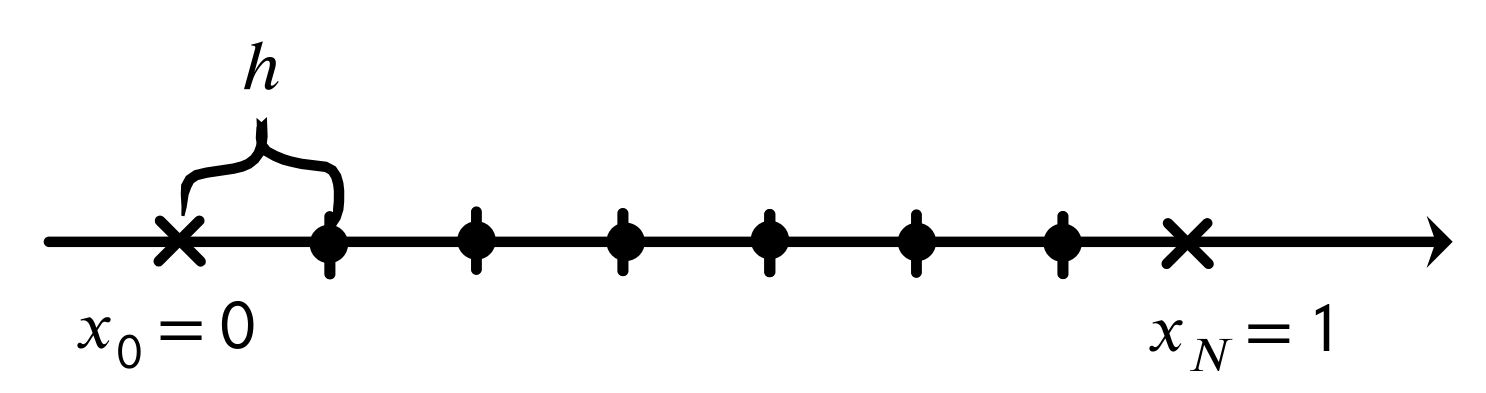
\includegraphics[scale=0.5]{img001}
    $$
    На этой сетке определим сеточную функцию $y = y(x)$, которая будет являться приближенным решением поставленной задачи (1), то есть это будет сеточное приближение функции $u = u(x)$.
    \\\\
    Заменяя дифференциальные производные разностными, можем построить разностную схему в безиндексной форме
    \begin{equation}
    	\begin{dcases}
    		\left(k\left(x - \dfrac h2\right) y(x)_{\overline x}\right)_x - q(x) y(x) = -f(x),\ x \in \omega_h,\\
    		y(0) = \mu_1,\\
    		-y_{\overline x}(1) = \sigma_2 y(1).
    	\end{dcases}
    \end{equation}
    Если мы распишем все разностные производные, то получим разностную схему в индексной форме
    \begin{equation}
    	\begin{dcases}
    		\dfrac{k_{i+\frac12}y_{i+1} - k_{i+\frac12} y_i -k_{i-\frac12} y_i + k_{i-\frac12} y_{i-1} }{h^2} - q(x_i) y_i = -f(x_i),\ i = \overline{1, N-1},\\
    		y_0 = \mu_1,\\
    		- \dfrac{y_N - y_{N-1}}{h} = \sigma_2 y_N
    	\end{dcases}
    \end{equation}
    Исследуем порядок аппроксимации дифференциальной задачи построенной разностной схемой. Сперва рассмотрим погрешность аппроксимации дифференциального уравнения
    $$
    \psi_{h}(x) = \left(k\left(x-\dfrac h2\right)u_{\overline x}\right)_x - q(x)u(x) + f(x)
    $$
    Учитывая, что
    $$\left(k\left(x-\dfrac h2\right)u_{\overline x}\right)_x = (k(x)u'(x))' - \dfrac{h^2}{8}k''(x)u''(x) + O(h^3),$$
    подставим в уравнение для погрешности и получим
    $$
    \psi_h(x) = (k(x)u'(x))' - \dfrac{h^2}{8}k''(x)u''(x) + O(h^3)- q(x)u(x) + f(x) = - \dfrac{h^2}{8}k''(x)u''(x) + O(h^3) = O(h^2).
    $$
    Таким образом, дифференциальное уравнение аппроксимируется на шаблоне со вторым порядком. \\\\
    Рассмотрим погрешность аппроксимации левого граничного условия. Так как на левой границе у нас отсутствует аппроксимация производной, то левое граничное условие аппроксимируется точно, то есть
    $$\nu_h(0) = u(0) - \mu_1 = 0.$$
    Рассмотрим погрешность аппроксимации правого граничного условия
    $$\nu_h(1) = -u_{\overline x}(1) - \sigma_2 u(1).$$
    Так как $$u_{\overline x}(x) = u'(x) - \dfrac h 2u''(x) + O(h^2),$$
    то
    $$\nu_h(1) = -u'(1) + \dfrac h 2u''(1) + O(h^2) - \sigma_2 u(1) = \dfrac h2 u''(1) + O(h^2) = O(h).$$
    Таким образом, правое граничное условие аппроксимируется с первым порядком. Тогда общий порядок аппроксимации дифференциальной задачи разностной схемой равен
    $$\Psi_h(x) = \psi_h(x) + \nu_h(0) + \nu_h(1) = O(h),$$
    то есть получили аппроксимацию первого порядка.\\\\
    Повысим порядок аппроксимации разностной схемы, не изменяя минимального шаблона. Поскольку мы получаем аппроксимацию первого порядка именно из-за правого граничного условия, то представим его в другом виде
    $$-y_{\overline x}(1) = \overline \sigma_2 y(1) + \overline \mu_2,$$
    где $\overline \sigma_2, \overline \mu _2$ -- это сеточные параметры, которые подлежат определению. Рассмотрим невязку над точным решением, чтобы определить вид введенных параметров
    $$\nu _h (1) = -u_{\overline x}(1) - \overline \sigma_2 u(1) - \overline \mu_2 = -u'(1) + \dfrac h 2 u''(1)+ O(h^2) - \overline \sigma_2 u(1)- \overline \mu_2.$$
    Предположим, что дифференциальное уравнение поставленной задачи (1) выполняется на правой границе, то есть
    $$(k(1)u'(1))' - q(1)u(1) = -f(1),$$
    тогда получим
    $$k'(1)u'(1) + k(1) u''(1) - q(1)u(1) = -f(1).$$
    Отсюда можем получить
    $$u''(1) = \dfrac {q(1)u(1) - f(1) - k'(1)u'(1)}{k(1)}.$$
    Таким образом, учитывая, что $-u'(1) = \sigma_2 u(1)$, получим
    $$\nu _h (1) = \sigma_2 u(1) + \dfrac h 2 \cdot\dfrac {q(1)u(1) - f(1) + k'(1)\sigma_2 u(1)}{k(1)} + O(h^2) - \overline \sigma_2 u(1)- \overline \mu_2.$$
    Тогда можно выбрать
    $$\begin{dcases}
    	\overline \sigma_2 = \sigma_2\cdot \left(1 + \dfrac h2 \cdot\dfrac { k'(1)}{ k(1)}\right) + \dfrac h 2 \cdot \dfrac {q(1)}{k(1)} ,\\
    	\overline \mu_2 = -\dfrac h 2 \cdot \dfrac {f(1)}{k(1)}.
    \end{dcases}$$
    При таком выборе мы получим аппроксимацию правого граничного условия со вторым порядком. Следовательно, вся дифференциальная задача будет аппроксимироваться со вторым порядком разностной схемой вида
    \begin{equation}
    	\begin{dcases}
    		\left(k\left(x - \dfrac h2\right) y(x)_{\overline x}\right)_x - q(x) y(x) = -f(x),\ x \in \omega_h,\\
    		y(0) = \mu_1,\\
    		-y_{\overline x}(1) =\left[\sigma_2\cdot \left(1 + \dfrac h2 \cdot\dfrac { k'(1)}{ k(1)}\right) + \dfrac h 2 \cdot \dfrac {q(1)}{k(1)} \right] y(1) - \dfrac h 2 \cdot \dfrac {f(1)}{k(1)}.
    	\end{dcases}
    \end{equation}
    Но для реализации разностной схемы нам нужна индексная форма записи
    \begin{equation}
    	\begin{dcases}
    		\dfrac{k_{i+\frac12}y_{i+1} - k_{i+\frac12} y_i -k_{i-\frac12} y_i + k_{i-\frac12} y_{i-1} }{h^2} - q(x_i) y_i = -f(x_i),\ i = \overline{1, N-1},\\
    		y_0 = \mu_1,\\
    		- \dfrac{y_N - y_{N-1}}{h} = \left[\sigma_2\cdot \left(1 + \dfrac h2 \cdot\dfrac { k'(1)}{ k(1)}\right) + \dfrac h 2 \cdot \dfrac {q(1)}{k(1)} \right] y_N - \dfrac h 2 \cdot \dfrac {f(1)}{k(1)}
    	\end{dcases}
    \end{equation}
    Чтобы применить к разностной схеме метод прогонки, выпишем коэффициенты, которые будут образовывать трехдиагональную матрицу. Если мы задаем трехдиагональную матрицу в виде
    \begin{equation}
    	\begin{pmatrix} 
    		\gamma_0 & \beta_0 & 0 & \ldots & 0 & 0 & \vrule & g_0 \\ 
    		\alpha_1 & \gamma_1 & \beta_1 & \ldots & 0 & 0 & \vrule & g_1\\ 
    		0 & \alpha_1 & \gamma_2 & \ldots & 0 & 0 & \vrule & g_2\\ 
    		\vdots & \vdots & \vdots & \ddots & \vdots & \vdots & \vrule & \vdots\\ 
    		0 & 0 & 0 & \ldots& \gamma_{N-1} & \beta_{N-1} & \vrule & g_{N-1} \\ 
    		0 & 0 & 0 & \ldots& \alpha_N& \gamma_N & \vrule & g_N\\\end{pmatrix}
    \end{equation}
    то
    в соответствии с нашей разностной схемой (6) имеем
    $$\gamma_0 = 1,\ \beta_0 = 0,\ g_0 = \mu_1,$$
    $$\alpha_i = \dfrac{k(x_i - \frac h2)}{h^2},\ \gamma_i = -\dfrac{k(x_i - \frac h2) + k(x_i + \frac h2)}{h^2} - q(x_i), \ \beta_i =\dfrac{k(x_i + \frac h2)}{h^2},\ g_i = -f(x_i),$$
    $$\alpha_N = \dfrac 1 h,\ \gamma_N = -\left[\dfrac 1h + \sigma_2\cdot \left(1 + \dfrac h2 \cdot\dfrac { k'(1)}{ k(1)}\right) + \dfrac h 2 \cdot \dfrac {q(1)}{k(1)}\right],\ g_N = - \dfrac h 2 \cdot \dfrac {f(1)}{k(1)}.$$
    Покажем, что в данном случае метод прогонки сходится. Для сходимости метода необходимо выполнение следующих условий:
    $$|\beta_0| \leq |\gamma _0|,\ |\alpha_i| + |\beta_i|\leq |\gamma_i|,\ |\alpha_N|\leq |\gamma_N|.$$
    Действительно,
    $$|\beta_0| \leq |\gamma _0| \Rightarrow 0 < 1,$$
    то есть первое условие верно, причем равенство строгое;
    $$|\alpha_i| + |\beta_i|\leq |\gamma_i|\Rightarrow \left|\dfrac{k(x_i - \frac h2)}{h^2} \right| + \left| \dfrac{k(x_i + \frac h2)}{h^2}\right|\leq \left|-\dfrac{k(x_i - \frac h2) + k(x_i + \frac h2)}{h^2} - q(x_i) \right|,$$
    оба выражения под модулями слева неотрицательны, так как являются сеточными функциями, а справа при раскрытии модуля меняем знак
    $$\dfrac{k(x_i - \frac h2)}{h^2}  +  \dfrac{k(x_i + \frac h2)}{h^2}\leq \dfrac{k(x_i - \frac h2) + k(x_i + \frac h2)}{h^2} + q(x_i),$$
    отсюда
    $$q(x_i)\geq 0,$$
    что верно для каждого $x_i$ из сетки;
    $$|\alpha_N|\leq |\gamma_N| \Rightarrow \left|\dfrac 1 h\right|\leq \left| -\left[\dfrac 1h + \sigma_2\cdot \left(1 + \dfrac h2 \cdot\dfrac { k'(1)}{ k(1)}\right) + \dfrac h 2 \cdot \dfrac {q(1)}{k(1)}\right]\right|,$$
    где при раскрытии модулей очевидно неравенство будет выполняться, так как справа мы прибавляем положительное число к $\dfrac 1 h$. Таким образом, метод прогони для реализации разностной схемы сходится.
    \section{Построение консервативной разностной схемы методом баланса}
    Для построения разностной схемы нам нужно привести поставленную задачу (1) к подходящему виду. В общем случае разностная схема по методу баланса строится для задачи вида 
    $$
    \begin{cases}
    	(k(x) u'(x))' - q(x)u(x) = -f(x), \ 0<x<1,\\
    	k(0) u'(0) = \sigma_1 u(0) - \mu_1,\\
    	- k(1) u'(1) = \sigma_2 u(1) - \mu_2.
    \end{cases}
    $$
    В нашей задаче граничные условия имеют другой вид, поэтому приведем их к нужному виду. Рассмотрим левое граничное условие. Если мы полагаем, что наше решение $u'(0) = 0$ и $\sigma_1 = 1$, то как раз получим левое граничное условие задачи (1):
    $$0 = u(0) - \mu_1 \Rightarrow u(0) = \mu_1,$$
    поэтому в левом граничном условии мы ничего менять не будем. В задаче у правого граничного условия есть множитель $k(1)$, который в нашем случае равен 
    $$k(1) = 4 - 1^2 = 3.$$
    Таким образом, мы должны домножить на это значение правое граничное условие, тогда
    $$-3 u'(1) = 3 \sigma_2 u(1).$$
    Таким образом, метод баланса мы будем применять к дифференциальной задаче
    \begin{equation}
    	\begin{cases}
    		(k(x)u'(x))' - q(x)u(x) = -f(x),\ 0 < x<1,\\
    		u(0) = \mu_1,\\
    		-3u'(1) = 3\sigma_2 u(1),
    	\end{cases}
    \end{equation}
    Из предыдущего пункта мы возьмем заданную равномерную сетку узлов $\overline \omega_h$ и заданную на ней сеточную функцию $y = y(x)$.
    \\\\
    По методу баланса можно построить разностную схему в безиндексном виде
    \begin{equation}
    	\begin{dcases}
    		(a y_{\overline x})_x - dy = -\varphi,\ x \in \omega_h, \\
    		a_1 y_{x,0} = \left(\sigma_0 + \dfrac h2 d_0\right)y_0 - \left(\mu_0 + \dfrac h2 \varphi_0\right),\\
    		-a_N y_{\overline x, N} = \left(\sigma_1 + \dfrac h2 d_N\right)y_N - \left(\mu_1 + \dfrac h2 \varphi_N\right);
    	\end{dcases}
    \end{equation}
    где 
    \begin{equation}
    	a_i = \left[ \dfrac 1h \int\limits_{x_{i-1}}^{x_i} \dfrac{1}{k(x)}dx\right]^{-1},\
    	d_i =\dfrac 1h \int\limits_{x_{i-\frac12}}^{x_{i+\frac12}} q(x) dx,\
    	\varphi_i = \dfrac{1}{h} \int\limits_{x_{i-\frac12}}^{x_{i+\frac12}}f(x)dx,
    \end{equation}
    \begin{equation}
    	d_0 = \dfrac2h \int\limits_0^{\frac h2}q(x)dx,\ \varphi_0 = \dfrac 2h \int\limits_0^{\frac h2}f(x)dx,
    \end{equation}
    \begin{equation}
    	d_N = \dfrac2h \int\limits_{1-\frac h2}^1 q(x)dx,\ \varphi_N = \dfrac 2h \int\limits_{1-\frac h2}^1f(x)dx.
    \end{equation}
    Или, что то же самое, в индексном виде
    \begin{equation}
    	\begin{dcases}
    		\dfrac{1}{h}\left(a_{i+1}\dfrac{y_{i+1} - y_i}{h} - a_i \dfrac{y_i - y_{i-1}}{h}\right)-d_iy_i = -\varphi_i,\ i=\overline {1,N-1}\\
    		a_1 y_{x,0} = \left(\sigma_0 + \dfrac h2 d_0\right)y_0 - \left(\mu_0 + \dfrac h2 \varphi_0\right),\\
    		-a_N y_{\overline x, N} = \left(\sigma_1 + \dfrac h2 d_N\right)y_N - \left(\mu_1 + \dfrac h2 \varphi_N\right);
    	\end{dcases}
    \end{equation}
    Для того, чтобы явно записать консервативную разностную схему для поставленной задачи (1), нам необходимо подогнать схему вида (11) под вид дифференциальной задачи (6) и вычислить коэффициенты по формулам (8), (9), (10). Причем будем строить наилучшую консервативную разностную схему, а значит интегралы будем вычислять точно.
    Итак, учитывая вид граничных условий задачи (6), получим разностную схему
    \begin{equation}
    	\begin{dcases}
    		\dfrac{1}{h}\left(a_{i+1}\dfrac{y_{i+1} - y_i}{h} - a_i \dfrac{y_i - y_{i-1}}{h}\right)-d_iy_i = -\varphi_i,\ i=\overline {1,N-1}\\
    		y_0 = \mu_1,\\
    		-a_N \dfrac{y_N - y_{N-1}}{h} = \left(3\sigma_2 + \dfrac h2 d_N\right)y_N - \dfrac h2 \varphi_N;
    	\end{dcases}
    \end{equation}
    в которой мы исключили аппроксимацию левого граничного условия, поскольку оно вычисляется точно. Определим коэффициенты, используя входные данные, 
    $$a_i = \left[ \dfrac 1h \int\limits_{x_{i-1}}^{x_i} \dfrac{dx}{4-x^2}\right]^{-1} = \left[ \dfrac 1h\cdot \dfrac 12 \ln \dfrac{2+x}{2-x}\Big|_{x_{i-1}}^{x_i}\right]^{-1} = \dfrac{2h}{\ln \dfrac{(2+x_i)(2-x_{i-1})}{(2-x_i)(2+x_{i-1})}},$$
    $$d_i=\dfrac 1h \int\limits_{x_{i-\frac12}}^{x_{i+\frac12}} x^2 dx = \dfrac 1 h\cdot \dfrac {x^3}{3}\Big | _{x_{i-\frac12}}^{x_{i+\frac12}}=\dfrac 1h\cdot \dfrac{(x_{i+\frac12}^3 - x_{i - \frac 12}^3)}{3},$$
    $$\varphi_i = \dfrac{1}{h} \int\limits_{x_{i-\frac12}}^{x_{i+\frac12}}[4\cos x - 2 x \sin x]dx = \dfrac 2 h (\sin x  + x \cos x)\Big | _{x_{i-\frac12}}^{x_{i+\frac12}}=$$ $$= \dfrac 2 h (\sin x_{i+\frac 12} - \sin x_{i-\frac 12} + x_{i+\frac 12}\cos x_{i+\frac 12} - x_{i-\frac 12}\cos x_{i-\frac 12}),$$
    $$d_N = \dfrac 2 h\cdot \dfrac {x^3}{3}\Big | _{1-\frac h 2}^{1} = \dfrac {2}{3h} - \dfrac{2 \left(1 - \frac h2\right)^3}{3h},$$ $$\varphi_N = \dfrac 4 h (\sin x  + x \cos x)\Big | _{1-\frac h2}^{1} = \dfrac 4 h \left(\sin 1 + \cos 1 - \sin \left(1-\dfrac h 2\right)- \left(1-\dfrac h 2\right) \cos \left(1-\dfrac h 2\right)\right).$$
    Таким образом, мы имеем общую формулу (12) для итераций и явные выражения для всех коэффициентов из этой разностной схемы. \\\\
    Полученная таким образом разностная схема обладает вторым порядком аппроксимации, а также для нее сходится метод прогонки.
    Запишем в соответствии с матрицей (7) вид коэффициентов для метода прогонки
    $$\gamma_0 = 1,\ \beta_0 = 0,\ g_0 = \mu_1,$$
    $$\alpha_i = \dfrac{a_i}{h^2},\ \gamma_i = -\dfrac{a_{i} + a_{i+1}}{h^2} - d_i, \ \beta_i =\dfrac{a_{i+1}}{h^2},\ g_i = -\varphi_i,$$
    $$\alpha_N = \dfrac{a_N} h,\ \gamma_N = -\left[\dfrac{a_N}{h} + 3\sigma_2 + \dfrac h2 d_N\right],\ g_N = - \dfrac h 2 \varphi_N.$$
    \section{Построение вариационно-разностной схемы методом Ритца}
    Из первого пункта мы возьмем заданную равномерную сетку узлов $\overline \omega_h$ и заданную на ней сеточную функцию $y = y(x)$.
    \\\\
    По методу Ритца мы можем построить трехдиагональную систему вида
    \begin{equation}
    	\begin{cases}
    		\alpha_{ii-1} y_{i-1} + \alpha_{ii} y_i + \alpha_{i i+1} y_{i+1} = \beta_i,\ i = \overline {1, N -1},\\
    		\alpha_{00} y_0 + \alpha_{01}y_1 = \beta_0,\\
    		\alpha_{NN-1} y_{N-1} + \alpha_{NN}y_N = \beta_N,
    	\end{cases}
    \end{equation}
    где $$\alpha_{ii} = \dfrac{1}{h^2}\left[ \int\limits_{x_{i-1}}^{x_{i+1}} k(x)dx +\int\limits_{x_{i-1}}^{x_i}q(x)(x-x_{i-1})^2dx + \int\limits_{x_i}^{x_{i+1}}q(x)(x_{i+1}-x)^2dx \right],\ i = \overline{1, N-1},$$
    $$\alpha_{ii+1} = \dfrac{1}{h^2} \left[-\int\limits_{x_i}^{x_{i+1}}k(x)dx + \int\limits_{x_i}^{x_{i+1}}q(x)(x-x_i)(x_{i+1} - x)dx\right],\ i = \overline {0, N-1},$$
    причем $\alpha_{ii+1} = \alpha_{i+1i}$. Тогда можно вычислить
    $$\beta_i = \dfrac{1}{h} \left[\int\limits_{x_{i-1}}^{x_i}f(x)(x-x_{i-1})dx + \int\limits_{x_i}^{x_{i+1}}f(x)(x_{i+1}-x)dx\right],\ i = \overline{1, N-1},$$
    $$\alpha_{00} = \dfrac{1}{h^2}\left[\int\limits_0^h k(x)dx + \int\limits_0^h q(x)(x-h)^2dx\right] + \sigma_1,$$
    $$\alpha_{NN} = \dfrac{1}{h^2}\left[\int\limits_{1-h}^1 k(x)dx + \int\limits_{1-h}^1 q(x)(x-1+h)^2dx\right] + \sigma_2,$$
    $$\beta_0 = \dfrac 1h \left[\int\limits_0^h f(x)(h-x)dx + \mu_1\right],\ \beta_N =  \dfrac{1}{h} \left[\int\limits_{1-h}^1 f(x)(x-1+h)dx + \mu_2\right].$$
    Нас интересуют граничные условия другого вида, поэтому мы будем вычислять
    $$a_i = -h\alpha_{ii-1},\ \varphi_i = \dfrac 1 h \beta_i,\ d_i = \dfrac 1h(\alpha_{ii-1} +\alpha_{ii} + \alpha_{ii+1}),$$
    $$d_0 = \dfrac{2}{h^2}\int\limits_0^h q(x)(h-x)dx,\ d_N = \dfrac{2}{h^2}\int\limits_{1-h}^1 q(x)(x-1+h)dx,$$
    $$\varphi_0 = \dfrac{2}{h^2}\int\limits_0^h f(x)(x-h)dx,\ \varphi_N=\dfrac{2}{h^2}\int\limits_{1-h}^1 f(x)(x-1+h)dx,$$
    откуда
    разностная схема будет иметь вид	
    \begin{equation*}
    	\begin{dcases}
    		\dfrac{a_i}{h^2}y_{i-1} - \left(\dfrac{a_i +a_{i+1}}{h}+d_i\right)y_i + \dfrac{a_{i+1}}{h^2}y_{i+1} = -\varphi_i,\ i=\overline {1,N-1}\\
    		a_1 y_{x,0} = \left(\sigma_0 + \dfrac h2 d_0\right)y_0 - \left(\mu_0 + \dfrac h2 \varphi_0\right),\\
    		-a_N y_{\overline x, N} = \left(\sigma_1 + \dfrac h2 d_N\right)y_N - \left(\mu_1 + \dfrac h2 \varphi_N\right);
    	\end{dcases}
    \end{equation*}
    но в нашем случае (по аналогии с методом баланса)
    \begin{equation}
    	\begin{dcases}
    		\dfrac{a_i}{h^2}y_{i-1} - \left(\dfrac{a_i +a_{i+1}}{h}+d_i\right)y_i + \dfrac{a_{i+1}}{h^2}y_{i+1} = -\varphi_i,\ i=\overline {1,N-1}\\
    		y_0 = \mu_1,\\
    		-a_N \dfrac{y_N - y_{N-1}}{h} = \left(3\sigma_2 + \dfrac h2 d_N\right)y_N - \dfrac h2 \varphi_N;
    	\end{dcases}
    \end{equation}
    Тогда, подставляя известные значения, получим
    $$\alpha_{ii} = \dfrac {1}{h^2}\left[ \left(4 x- \dfrac{x}{3}\right) \Big|_{x_{i-1}}^{x_{i+1}} + \left(\dfrac{x^5}{5} - \dfrac{x^4 x_{i-1}}{2} + \dfrac{x^3 x_{i-1}^2}{3}\right)\Big|_{x_{i-1}}^{x_i} + \left(\dfrac{x^5}{5} - \dfrac{x^4 x_{i+1}}{2} + \dfrac{x^3 x_{i+1}^2}{3}\right)\Big|_{x_{i}}^{x_{i+1}}\right],$$
    $$\alpha_{ii+1} = \dfrac{1}{h^2}\left[-\left(4 x- \dfrac{x}{3}\right) \Big|_{x_{i}}^{x_{i+1}} + \left(\dfrac{x^4(x_i + x_{i+1})}{4}-\dfrac 1 3 x_i x_{i+1}x^3 - \dfrac{x^5}{5}\right)\Big|_{x_{i}}^{x_{i+1}}\right],$$
    $$\alpha_{ii-1} = \dfrac{1}{h^2}\left[-\left(4 x- \dfrac{x}{3}\right) \Big|_{x_{i-1}}^{x_{i}} + \left(\dfrac{x^4(x_{i-1} + x_{i})}{4}-\dfrac 1 3 x_{i-1} x_{i}x^3 - \dfrac{x^5}{5}\right)\Big|_{x_{i-1}}^{x_{i}}\right],$$
    $$\beta_i = \dfrac 1 h \left[-2(x_{i-1}\sin x - x (x - x_{i-1})\cos x)\Big|_{x_{i-1}}^{x_i} + 2(x_{i+1}\sin x + x (x_{i+1} - x)\cos x)\Big|_{x_{i}}^{x_{i+1}}\right],$$
    $$ d_N = \dfrac{2}{12h^2}\left[x^3\cdot (4h+3x-4) \right]\Big|_{1-h}^{1},$$
    $$\varphi_N = \dfrac{2}{h^2} \left[2(h-1)\sin x + 2x(h+x-1)\cos x\right]\Big|_{1-h}^{1}.$$
    Полученная таким образом разностная схема обладает вторым порядком аппроксимации, а также для нее сходится метод прогонки.\\\\
    Для нее коэффициенты метода прогонки возьмем такие же, как и в предыдущем случае, поскольку мы привели разностную схему к такому же виду, как для метода баланса.
    
    \section{Реализация на ЭВМ}

    
    Подключим все необходимые библиотеки для вычислений и для визуализации

    \begin{tcolorbox}[breakable, size=fbox, boxrule=1pt, pad at break*=1mm,colback=cellbackground, colframe=cellborder]
\prompt{In}{incolor}{1}{\boxspacing}
\begin{Verbatim}[commandchars=\\\{\}]
\PY{k+kn}{import} \PY{n+nn}{numpy} \PY{k}{as} \PY{n+nn}{np}
\PY{k+kn}{import} \PY{n+nn}{math}
\PY{k+kn}{import} \PY{n+nn}{matplotlib}\PY{n+nn}{.}\PY{n+nn}{pyplot} \PY{k}{as} \PY{n+nn}{plt}
\end{Verbatim}
\end{tcolorbox}

    Определим функцию для решения системы с трехдиагональной матрицей

    \begin{tcolorbox}[breakable, size=fbox, boxrule=1pt, pad at break*=1mm,colback=cellbackground, colframe=cellborder]
\prompt{In}{incolor}{2}{\boxspacing}
\begin{Verbatim}[commandchars=\\\{\}]
\PY{k}{def} \PY{n+nf}{tridiagonal\PYZus{}algorithm}\PY{p}{(}\PY{n}{a}\PY{p}{,}\PY{n}{b}\PY{p}{,}\PY{n}{c}\PY{p}{,}\PY{n}{f}\PY{p}{)}\PY{p}{:}
    \PY{n}{a}\PY{p}{,} \PY{n}{b}\PY{p}{,} \PY{n}{c}\PY{p}{,} \PY{n}{f} \PY{o}{=} \PY{n+nb}{tuple}\PY{p}{(}\PY{n+nb}{map}\PY{p}{(}\PY{k}{lambda} \PY{n}{k\PYZus{}list}\PY{p}{:} \PY{n+nb}{list}\PY{p}{(}\PY{n+nb}{map}\PY{p}{(}\PY{n+nb}{float}\PY{p}{,} \PY{n}{k\PYZus{}list}\PY{p}{)}\PY{p}{)}\PY{p}{,} \PY{p}{(}\PY{n}{a}\PY{p}{,} \PY{n}{b}\PY{p}{,} \PY{n}{c}\PY{p}{,} \PY{n}{f}\PY{p}{)}\PY{p}{)}\PY{p}{)}

    \PY{n}{alpha} \PY{o}{=} \PY{p}{[}\PY{o}{\PYZhy{}}\PY{n}{b}\PY{p}{[}\PY{l+m+mi}{0}\PY{p}{]} \PY{o}{/} \PY{n}{c}\PY{p}{[}\PY{l+m+mi}{0}\PY{p}{]}\PY{p}{]}
    \PY{n}{beta} \PY{o}{=} \PY{p}{[}\PY{n}{f}\PY{p}{[}\PY{l+m+mi}{0}\PY{p}{]} \PY{o}{/} \PY{n}{c}\PY{p}{[}\PY{l+m+mi}{0}\PY{p}{]}\PY{p}{]}
    \PY{n}{n} \PY{o}{=} \PY{n+nb}{len}\PY{p}{(}\PY{n}{f}\PY{p}{)}
    \PY{n}{x} \PY{o}{=} \PY{p}{[}\PY{l+m+mi}{0}\PY{p}{]}\PY{o}{*}\PY{n}{n}

    \PY{k}{for} \PY{n}{i} \PY{o+ow}{in} \PY{n+nb}{range}\PY{p}{(}\PY{l+m+mi}{1}\PY{p}{,} \PY{n}{n}\PY{p}{)}\PY{p}{:}
        \PY{n}{alpha}\PY{o}{.}\PY{n}{append}\PY{p}{(}\PY{o}{\PYZhy{}}\PY{n}{b}\PY{p}{[}\PY{n}{i}\PY{p}{]}\PY{o}{/}\PY{p}{(}\PY{n}{a}\PY{p}{[}\PY{n}{i}\PY{p}{]}\PY{o}{*}\PY{n}{alpha}\PY{p}{[}\PY{n}{i}\PY{o}{\PYZhy{}}\PY{l+m+mi}{1}\PY{p}{]} \PY{o}{+} \PY{n}{c}\PY{p}{[}\PY{n}{i}\PY{p}{]}\PY{p}{)}\PY{p}{)}
        \PY{n}{beta}\PY{o}{.}\PY{n}{append}\PY{p}{(}\PY{p}{(}\PY{n}{f}\PY{p}{[}\PY{n}{i}\PY{p}{]} \PY{o}{\PYZhy{}} \PY{n}{a}\PY{p}{[}\PY{n}{i}\PY{p}{]}\PY{o}{*}\PY{n}{beta}\PY{p}{[}\PY{n}{i}\PY{o}{\PYZhy{}}\PY{l+m+mi}{1}\PY{p}{]}\PY{p}{)}\PY{o}{/}\PY{p}{(}\PY{n}{a}\PY{p}{[}\PY{n}{i}\PY{p}{]}\PY{o}{*}\PY{n}{alpha}\PY{p}{[}\PY{n}{i}\PY{o}{\PYZhy{}}\PY{l+m+mi}{1}\PY{p}{]} \PY{o}{+} \PY{n}{c}\PY{p}{[}\PY{n}{i}\PY{p}{]}\PY{p}{)}\PY{p}{)}

    \PY{n}{x}\PY{p}{[}\PY{n}{n}\PY{o}{\PYZhy{}}\PY{l+m+mi}{1}\PY{p}{]} \PY{o}{=} \PY{n}{beta}\PY{p}{[}\PY{n}{n} \PY{o}{\PYZhy{}} \PY{l+m+mi}{1}\PY{p}{]}

    \PY{k}{for} \PY{n}{i} \PY{o+ow}{in} \PY{n+nb}{range}\PY{p}{(}\PY{n}{n} \PY{o}{\PYZhy{}} \PY{l+m+mi}{1}\PY{p}{,} \PY{l+m+mi}{0}\PY{p}{,} \PY{o}{\PYZhy{}}\PY{l+m+mi}{1}\PY{p}{)}\PY{p}{:}
        \PY{n}{x}\PY{p}{[}\PY{n}{i} \PY{o}{\PYZhy{}} \PY{l+m+mi}{1}\PY{p}{]} \PY{o}{=} \PY{n}{alpha}\PY{p}{[}\PY{n}{i} \PY{o}{\PYZhy{}} \PY{l+m+mi}{1}\PY{p}{]}\PY{o}{*}\PY{n}{x}\PY{p}{[}\PY{n}{i}\PY{p}{]} \PY{o}{+} \PY{n}{beta}\PY{p}{[}\PY{n}{i} \PY{o}{\PYZhy{}} \PY{l+m+mi}{1}\PY{p}{]}

    \PY{k}{return} \PY{n}{x}
\end{Verbatim}
\end{tcolorbox}

    В соответствии с входными данными определим функции:

\begin{itemize}
\item
  \(k(x) = 4-x^2\) -- это коэффициент теплопроводности материала
  стержня;
\item
  \(q(x) = x^2\) отвечает за мощность стоков или источников тепла;
\item
  \(f(x)=4\cos x - 2 x\sin x\) -- это плотность распределения внешних
  источников или стоков тепла;
\item
  \(\mu_1 = 1\);
\item
  \(\sigma_2 = \tan 1\);
\end{itemize}

Также нам понадобится функция

\begin{itemize}
\tightlist
\item
  \(k'(x) = -2x\).
\end{itemize}

    \begin{tcolorbox}[breakable, size=fbox, boxrule=1pt, pad at break*=1mm,colback=cellbackground, colframe=cellborder]
\prompt{In}{incolor}{4}{\boxspacing}
\begin{Verbatim}[commandchars=\\\{\}]
\PY{k}{def} \PY{n+nf}{k}\PY{p}{(}\PY{n}{x}\PY{p}{)}\PY{p}{:}
    \PY{k}{return} \PY{l+m+mi}{4} \PY{o}{\PYZhy{}} \PY{n}{x}\PY{o}{*}\PY{o}{*}\PY{l+m+mi}{2}

\PY{k}{def} \PY{n+nf}{dkdx}\PY{p}{(}\PY{n}{x}\PY{p}{)}\PY{p}{:}
    \PY{k}{return} \PY{o}{\PYZhy{}}\PY{l+m+mi}{2}\PY{o}{*}\PY{n}{x}

\PY{k}{def} \PY{n+nf}{q}\PY{p}{(}\PY{n}{x}\PY{p}{)}\PY{p}{:}
    \PY{k}{return} \PY{n}{x}\PY{o}{*}\PY{o}{*}\PY{l+m+mi}{2}

\PY{k}{def} \PY{n+nf}{f}\PY{p}{(}\PY{n}{x}\PY{p}{)}\PY{p}{:}
    \PY{k}{return} \PY{l+m+mi}{4}\PY{o}{*}\PY{n}{np}\PY{o}{.}\PY{n}{cos}\PY{p}{(}\PY{n}{x}\PY{p}{)} \PY{o}{\PYZhy{}} \PY{l+m+mi}{2}\PY{o}{*}\PY{n}{x}\PY{o}{*}\PY{n}{np}\PY{o}{.}\PY{n}{sin}\PY{p}{(}\PY{n}{x}\PY{p}{)}

\PY{n}{mu\PYZus{}1} \PY{o}{=} \PY{l+m+mi}{1}
\PY{n}{sigma\PYZus{}2} \PY{o}{=} \PY{n}{np}\PY{o}{.}\PY{n}{tan}\PY{p}{(}\PY{l+m+mi}{1}\PY{p}{)}
\end{Verbatim}
\end{tcolorbox}

    Определим функцию, соответствующую точному решению дифференциальной
задачи \[u(x) = \cos x\]

    \begin{tcolorbox}[breakable, size=fbox, boxrule=1pt, pad at break*=1mm,colback=cellbackground, colframe=cellborder]
\prompt{In}{incolor}{30}{\boxspacing}
\begin{Verbatim}[commandchars=\\\{\}]
\PY{k}{def} \PY{n+nf}{u}\PY{p}{(}\PY{n}{x}\PY{p}{)}\PY{p}{:}
    \PY{k}{return} \PY{n}{np}\PY{o}{.}\PY{n}{cos}\PY{p}{(}\PY{n}{x}\PY{p}{)}
\end{Verbatim}
\end{tcolorbox}

    Определим сетку узлов \(\omega_h\) следующим образом: пусть
\([a,b] = [0,1]\), а число разбиений отрезка \(N = 5\).

    \begin{tcolorbox}[breakable, size=fbox, boxrule=1pt, pad at break*=1mm,colback=cellbackground, colframe=cellborder]
\prompt{In}{incolor}{31}{\boxspacing}
\begin{Verbatim}[commandchars=\\\{\}]
\PY{n}{a}\PY{p}{,} \PY{n}{b} \PY{o}{=} \PY{l+m+mi}{0}\PY{p}{,} \PY{l+m+mi}{1}
\PY{n}{N} \PY{o}{=} \PY{l+m+mi}{5}
\PY{n}{x} \PY{o}{=} \PY{n}{np}\PY{o}{.}\PY{n}{linspace}\PY{p}{(}\PY{n}{start}\PY{o}{=}\PY{n}{a}\PY{p}{,} \PY{n}{stop}\PY{o}{=}\PY{n}{b}\PY{p}{,} \PY{n}{num}\PY{o}{=}\PY{n}{N}\PY{o}{+}\PY{l+m+mi}{1}\PY{p}{)}
\PY{n}{h} \PY{o}{=} \PY{p}{(}\PY{n}{b}\PY{o}{\PYZhy{}}\PY{n}{a}\PY{p}{)}\PY{o}{/}\PY{n}{N}
\end{Verbatim}
\end{tcolorbox}

    \hypertarget{ux440ux430ux437ux43dux43eux441ux442ux43dux430ux44f-ux430ux43fux43fux440ux43eux43aux441ux438ux43cux430ux446ux438ux44f}{%
\subsection{Разностная
аппроксимация}\label{ux440ux430ux437ux43dux43eux441ux442ux43dux430ux44f-ux430ux43fux43fux440ux43eux43aux441ux438ux43cux430ux446ux438ux44f}}

    Итак, у нас есть разностная схема \[\begin{dcases}
            \dfrac{k_{i+\frac12}y_{i+1} - k_{i+\frac12} y_i -k_{i-\frac12} y_i + k_{i-\frac12} y_{i-1} }{h^2} - q(x_i) y_i = -f(x_i),\ i = \overline{1, N-1},\\
            y_0 = \mu_1,\\
            - \dfrac{y_N - y_{N-1}}{h} = \left[\sigma_2\cdot \left(1 + \dfrac h2 \cdot\dfrac { k'(1)}{ k(1)}\right) + \dfrac h 2 \cdot \dfrac {q(1)}{k(1)} \right] y_N - \dfrac h 2 \cdot \dfrac {f(1)}{k(1)}
        \end{dcases}\] Чтобы найти с помощью нее приближенное решение
дифференциальной задачи, нам нужно преобразовать эту разностную схему к
задаче на решение системы с трехиадогнальной матрицей. Таким образом,
задача на решение системы уравнений примет вид \[
        \begin{pmatrix} 
            \gamma_0 & \beta_0 & 0 & \ldots & 0 & 0 & \vrule & g_0 \\ 
            \alpha_1 & \gamma_1 & \beta_1 & \ldots & 0 & 0 & \vrule & g_1\\ 
            0 & \alpha_1 & \gamma_2 & \ldots & 0 & 0 & \vrule & g_2\\ 
            \vdots & \vdots & \vdots & \ddots & \vdots & \vdots & \vrule & \vdots\\ 
            0 & 0 & 0 & \ldots& \gamma_{N-1} & \beta_{N-1} & \vrule & g_{N-1} \\ 
            0 & 0 & 0 & \ldots& \alpha_N& \gamma_N & \vrule & g_N\\\end{pmatrix}
\] где \[\gamma_0 = 1,\ \beta_0 = 0,\ g_0 = \mu_1,\]
\[\alpha_i = \dfrac{k(x_i - \frac h2)}{h^2},\ \gamma_i = -\dfrac{k(x_i - \frac h2) + k(x_i + \frac h2)}{h^2} - q(x_i), \ \beta_i =\dfrac{k(x_i + \frac h2)}{h^2},\ g_i = -f(x_i),\]
\[\alpha_N = \dfrac 1 h,\ \gamma_N = -\left[\dfrac 1h + \sigma_2\cdot \left(1 + \dfrac h2 \cdot\dfrac { k'(1)}{ k(1)}\right) + \dfrac h 2 \cdot \dfrac {q(1)}{k(1)}\right],\ g_N = - \dfrac h 2 \cdot \dfrac {f(1)}{k(1)}.\]
Реализуем вычисление всех коэффициентов:

    \begin{tcolorbox}[breakable, size=fbox, boxrule=1pt, pad at break*=1mm,colback=cellbackground, colframe=cellborder]
\prompt{In}{incolor}{36}{\boxspacing}
\begin{Verbatim}[commandchars=\\\{\}]
\PY{n}{gamma} \PY{o}{=} \PY{p}{[}\PY{l+m+mi}{1}\PY{p}{]}
\PY{n}{beta} \PY{o}{=} \PY{p}{[}\PY{l+m+mi}{0}\PY{p}{]}
\PY{n}{g} \PY{o}{=} \PY{p}{[}\PY{n}{mu\PYZus{}1}\PY{p}{]}
\PY{n}{alpha} \PY{o}{=} \PY{p}{[}\PY{l+m+mi}{0}\PY{p}{]}
\PY{k}{for} \PY{n}{i} \PY{o+ow}{in} \PY{n+nb}{range}\PY{p}{(}\PY{l+m+mi}{1}\PY{p}{,} \PY{n}{N}\PY{p}{)}\PY{p}{:}
    \PY{n}{alpha}\PY{o}{.}\PY{n}{append}\PY{p}{(}\PY{n}{k}\PY{p}{(}\PY{n}{x}\PY{p}{[}\PY{n}{i}\PY{p}{]} \PY{o}{\PYZhy{}} \PY{n}{h}\PY{o}{/}\PY{l+m+mi}{2}\PY{p}{)} \PY{o}{/} \PY{n}{h}\PY{o}{*}\PY{o}{*}\PY{l+m+mi}{2}\PY{p}{)}
    \PY{n}{gamma}\PY{o}{.}\PY{n}{append}\PY{p}{(}\PY{o}{\PYZhy{}}\PY{p}{(}\PY{n}{k}\PY{p}{(}\PY{n}{x}\PY{p}{[}\PY{n}{i}\PY{p}{]} \PY{o}{\PYZhy{}} \PY{n}{h}\PY{o}{/}\PY{l+m+mi}{2}\PY{p}{)} \PY{o}{+} \PY{n}{k}\PY{p}{(}\PY{n}{x}\PY{p}{[}\PY{n}{i}\PY{p}{]} \PY{o}{+} \PY{n}{h}\PY{o}{/}\PY{l+m+mi}{2}\PY{p}{)}\PY{p}{)} \PY{o}{/} \PY{n}{h}\PY{o}{*}\PY{o}{*}\PY{l+m+mi}{2} \PY{o}{\PYZhy{}} \PY{n}{q}\PY{p}{(}\PY{n}{x}\PY{p}{[}\PY{n}{i}\PY{p}{]}\PY{p}{)}\PY{p}{)}
    \PY{n}{beta}\PY{o}{.}\PY{n}{append}\PY{p}{(}\PY{n}{k}\PY{p}{(}\PY{n}{x}\PY{p}{[}\PY{n}{i}\PY{p}{]} \PY{o}{+} \PY{n}{h}\PY{o}{/}\PY{l+m+mi}{2}\PY{p}{)} \PY{o}{/} \PY{n}{h}\PY{o}{*}\PY{o}{*}\PY{l+m+mi}{2}\PY{p}{)}
    \PY{n}{g}\PY{o}{.}\PY{n}{append}\PY{p}{(}\PY{o}{\PYZhy{}}\PY{n}{f}\PY{p}{(}\PY{n}{x}\PY{p}{[}\PY{n}{i}\PY{p}{]}\PY{p}{)}\PY{p}{)}
\PY{n}{alpha}\PY{o}{.}\PY{n}{append}\PY{p}{(}\PY{l+m+mi}{1}\PY{o}{/}\PY{n}{h}\PY{p}{)}
\PY{n}{gamma}\PY{o}{.}\PY{n}{append}\PY{p}{(}\PY{o}{\PYZhy{}} \PY{p}{(}\PY{l+m+mi}{1}\PY{o}{/}\PY{n}{h} \PY{o}{+} \PY{n}{sigma\PYZus{}2} \PY{o}{*} \PY{p}{(}\PY{l+m+mi}{1} \PY{o}{+} \PY{n}{h}\PY{o}{/}\PY{l+m+mi}{2} \PY{o}{*} \PY{n}{dkdx}\PY{p}{(}\PY{l+m+mi}{1}\PY{p}{)} \PY{o}{/} \PY{n}{k}\PY{p}{(}\PY{l+m+mi}{1}\PY{p}{)}\PY{p}{)} \PY{o}{+} \PY{n}{h}\PY{o}{/}\PY{l+m+mi}{2} \PY{o}{*} \PY{n}{q}\PY{p}{(}\PY{l+m+mi}{1}\PY{p}{)} \PY{o}{/} \PY{n}{k}\PY{p}{(}\PY{l+m+mi}{1}\PY{p}{)}\PY{p}{)}\PY{p}{)}
\PY{n}{g}\PY{o}{.}\PY{n}{append}\PY{p}{(}\PY{o}{\PYZhy{}}\PY{n}{h}\PY{o}{/}\PY{l+m+mi}{2} \PY{o}{*} \PY{n}{f}\PY{p}{(}\PY{l+m+mi}{1}\PY{p}{)} \PY{o}{/} \PY{n}{k}\PY{p}{(}\PY{l+m+mi}{1}\PY{p}{)}\PY{p}{)}
\PY{n}{beta}\PY{o}{.}\PY{n}{append}\PY{p}{(}\PY{l+m+mi}{0}\PY{p}{)}
\end{Verbatim}
\end{tcolorbox}

    Теперь определим приближенное решение разностной задачи как решение
системы с трехдиагональной матрицей

    \begin{tcolorbox}[breakable, size=fbox, boxrule=1pt, pad at break*=1mm,colback=cellbackground, colframe=cellborder]
\prompt{In}{incolor}{37}{\boxspacing}
\begin{Verbatim}[commandchars=\\\{\}]
\PY{n}{y} \PY{o}{=} \PY{n}{tridiagonal\PYZus{}algorithm}\PY{p}{(}\PY{n}{alpha}\PY{p}{,}\PY{n}{beta}\PY{p}{,}\PY{n}{gamma}\PY{p}{,}\PY{n}{g}\PY{p}{)}
\end{Verbatim}
\end{tcolorbox}

    Визуализируем полученные результаты

    \begin{tcolorbox}[breakable, size=fbox, boxrule=1pt, pad at break*=1mm,colback=cellbackground, colframe=cellborder]
\prompt{In}{incolor}{38}{\boxspacing}
\begin{Verbatim}[commandchars=\\\{\}]
\PY{n}{plt}\PY{o}{.}\PY{n}{figure}\PY{p}{(}\PY{n}{figsize}\PY{o}{=}\PY{p}{(}\PY{l+m+mi}{16}\PY{p}{,} \PY{l+m+mi}{8}\PY{p}{)}\PY{p}{)}
\PY{n}{plt}\PY{o}{.}\PY{n}{plot}\PY{p}{(}\PY{n}{x}\PY{p}{,} \PY{n}{u}\PY{p}{(}\PY{n}{x}\PY{p}{)}\PY{p}{,} \PY{n}{label}\PY{o}{=}\PY{l+s+s1}{\PYZsq{}}\PY{l+s+s1}{exact temperature}\PY{l+s+s1}{\PYZsq{}}\PY{p}{)}
\PY{n}{plt}\PY{o}{.}\PY{n}{plot}\PY{p}{(}\PY{n}{x}\PY{p}{,} \PY{n}{y}\PY{p}{,} \PY{n}{label}\PY{o}{=}\PY{l+s+s1}{\PYZsq{}}\PY{l+s+s1}{numerical temperature}\PY{l+s+s1}{\PYZsq{}}\PY{p}{)}
\PY{n}{plt}\PY{o}{.}\PY{n}{title}\PY{p}{(}\PY{l+s+s1}{\PYZsq{}}\PY{l+s+s1}{Аппроксимация разностными производными}\PY{l+s+s1}{\PYZsq{}}\PY{p}{)}
\PY{n}{plt}\PY{o}{.}\PY{n}{grid}\PY{p}{(}\PY{k+kc}{True}\PY{p}{)}
\PY{n}{plt}\PY{o}{.}\PY{n}{xlabel}\PY{p}{(}\PY{l+s+s1}{\PYZsq{}}\PY{l+s+s1}{x}\PY{l+s+s1}{\PYZsq{}}\PY{p}{)}
\PY{n}{plt}\PY{o}{.}\PY{n}{ylabel}\PY{p}{(}\PY{l+s+s1}{\PYZsq{}}\PY{l+s+s1}{u(x)}\PY{l+s+s1}{\PYZsq{}}\PY{p}{)}
\PY{n}{plt}\PY{o}{.}\PY{n}{legend}\PY{p}{(}\PY{p}{)}
\PY{n}{plt}\PY{o}{.}\PY{n}{show}\PY{p}{(}\PY{p}{)}
\end{Verbatim}
\end{tcolorbox}

    \begin{center}
    \adjustimage{max size={0.9\linewidth}{0.9\paperheight}}{output_16_0.png}
    \end{center}
    { \hspace*{\fill} \\}
    
    Как можно видеть из графика, приближенное решение максимально близко
описывает точное решение задачи.

    \hypertarget{ux43cux435ux442ux43eux434-ux431ux430ux43bux430ux43dux441ux430}{%
\subsection{Метод
баланса}\label{ux43cux435ux442ux43eux434-ux431ux430ux43bux430ux43dux441ux430}}

    Итак, у нас есть разностная схема \[
\begin{dcases}
            \dfrac{1}{h}\left(a_{i+1}\dfrac{y_{i+1} - y_i}{h} - a_i \dfrac{y_i - y_{i-1}}{h}\right)-d_iy_i = -\varphi_i,\ i=\overline {1,N-1}\\
            y_0 = \mu_1,\\
            -a_N \dfrac{y_N - y_{N-1}}{h} = \left(3\sigma_2 + \dfrac h2 d_N\right)y_N - \dfrac h2 \varphi_N;
        \end{dcases}
\] где
\[a_i = \left[ \dfrac 1h \int\limits_{x_{i-1}}^{x_i} \dfrac{dx}{4-x^2}\right]^{-1} = \left[ \dfrac 1h\cdot \dfrac 12 \ln \dfrac{2+x}{2-x}\Big|_{x_{i-1}}^{x_i}\right]^{-1} = \dfrac{2h}{\ln \dfrac{(2+x_i)(2-x_{i-1})}{(2-x_i)(2+x_{i-1})}},\]
\[d_i=\dfrac 1h \int\limits_{x_{i-\frac12}}^{x_{i+\frac12}} x^2 dx = \dfrac 1 h\cdot \dfrac {x^3}{3}\Big | _{x_{i-\frac12}}^{x_{i+\frac12}}=\dfrac 1h\cdot \dfrac{(x_{i+\frac12}^3 - x_{i - \frac 12}^3)}{3},\]
\[\varphi_i = \dfrac{1}{h} \int\limits_{x_{i-\frac12}}^{x_{i+\frac12}}[4\cos x - 2 x \sin x]dx = \dfrac 2 h (\sin x  + x \cos x)\Big | _{x_{i-\frac12}}^{x_{i+\frac12}}=\]
\[= \dfrac 2 h (\sin x_{i+\frac 12} - \sin x_{i-\frac 12} + x_{i+\frac 12}\cos x_{i+\frac 12} - x_{i-\frac 12}\cos x_{i-\frac 12}),\]
\[d_N = \dfrac 2 h\cdot \dfrac {x^3}{3}\Big | _{1-\frac h 2}^{1} = \dfrac {2}{3h} - \dfrac{2 \left(1 - \frac h2\right)^3}{3h},\]
\[\varphi_N = \dfrac 4 h (\sin x  + x \cos x)\Big | _{1-\frac h2}^{1} = \dfrac 4 h \left(\sin 1 + \cos 1 - \sin \left(1-\dfrac h 2\right)- \left(1-\dfrac h 2\right) \cos \left(1-\dfrac h 2\right)\right).\]
Определим функции для вычисления коэффициентов

    \begin{tcolorbox}[breakable, size=fbox, boxrule=1pt, pad at break*=1mm,colback=cellbackground, colframe=cellborder]
\prompt{In}{incolor}{46}{\boxspacing}
\begin{Verbatim}[commandchars=\\\{\}]
\PY{k}{def} \PY{n+nf}{a\PYZus{}i}\PY{p}{(}\PY{n}{x}\PY{p}{,} \PY{n}{h}\PY{p}{)}\PY{p}{:}
    \PY{k}{return} \PY{l+m+mi}{2} \PY{o}{*} \PY{n}{h} \PY{o}{/} \PY{n}{np}\PY{o}{.}\PY{n}{log}\PY{p}{(}\PY{p}{(}\PY{l+m+mi}{2}\PY{o}{+}\PY{n}{x}\PY{p}{)}\PY{o}{*}\PY{p}{(}\PY{l+m+mi}{2}\PY{o}{\PYZhy{}}\PY{p}{(}\PY{n}{x}\PY{o}{\PYZhy{}}\PY{n}{h}\PY{p}{)}\PY{p}{)} \PY{o}{/} \PY{p}{(}\PY{p}{(}\PY{l+m+mi}{2}\PY{o}{\PYZhy{}}\PY{n}{x}\PY{p}{)}\PY{o}{*}\PY{p}{(}\PY{l+m+mi}{2}\PY{o}{+}\PY{p}{(}\PY{n}{x}\PY{o}{\PYZhy{}}\PY{n}{h}\PY{p}{)}\PY{p}{)}\PY{p}{)}\PY{p}{)}

\PY{k}{def} \PY{n+nf}{d\PYZus{}i}\PY{p}{(}\PY{n}{x}\PY{p}{,} \PY{n}{h}\PY{p}{)}\PY{p}{:}
    \PY{k}{return} \PY{p}{(}\PY{p}{(}\PY{n}{x}\PY{o}{+}\PY{n}{h}\PY{o}{/}\PY{l+m+mi}{2}\PY{p}{)}\PY{o}{*}\PY{o}{*}\PY{l+m+mi}{3} \PY{o}{\PYZhy{}} \PY{p}{(}\PY{n}{x}\PY{o}{\PYZhy{}}\PY{n}{h}\PY{o}{/}\PY{l+m+mi}{2}\PY{p}{)}\PY{o}{*}\PY{o}{*}\PY{l+m+mi}{3}\PY{p}{)}\PY{o}{/}\PY{p}{(}\PY{l+m+mi}{3}\PY{o}{*}\PY{n}{h}\PY{p}{)} 

\PY{k}{def} \PY{n+nf}{phi\PYZus{}i}\PY{p}{(}\PY{n}{x}\PY{p}{,} \PY{n}{h}\PY{p}{)}\PY{p}{:}
    \PY{k}{return} \PY{l+m+mi}{2}\PY{o}{/}\PY{n}{h} \PY{o}{*} \PY{p}{(}\PY{n}{np}\PY{o}{.}\PY{n}{sin}\PY{p}{(}\PY{n}{x}\PY{o}{+}\PY{n}{h}\PY{o}{/}\PY{l+m+mi}{2}\PY{p}{)} \PY{o}{\PYZhy{}} \PY{n}{np}\PY{o}{.}\PY{n}{sin}\PY{p}{(}\PY{n}{x}\PY{o}{\PYZhy{}}\PY{n}{h}\PY{o}{/}\PY{l+m+mi}{2}\PY{p}{)} \PY{o}{+} \PY{p}{(}\PY{n}{x}\PY{o}{+}\PY{n}{h}\PY{o}{/}\PY{l+m+mi}{2}\PY{p}{)}\PY{o}{*}\PY{n}{np}\PY{o}{.}\PY{n}{cos}\PY{p}{(}\PY{n}{x}\PY{o}{+}\PY{n}{h}\PY{o}{/}\PY{l+m+mi}{2}\PY{p}{)} \PY{o}{\PYZhy{}} \PY{p}{(}\PY{n}{x}\PY{o}{\PYZhy{}}\PY{n}{h}\PY{o}{/}\PY{l+m+mi}{2}\PY{p}{)}\PY{o}{*}\PY{n}{np}\PY{o}{.}\PY{n}{cos}\PY{p}{(}\PY{n}{x}\PY{o}{\PYZhy{}}\PY{n}{h}\PY{o}{/}\PY{l+m+mi}{2}\PY{p}{)}\PY{p}{)}
                                                                                         
\PY{k}{def} \PY{n+nf}{d\PYZus{}N}\PY{p}{(}\PY{n}{h}\PY{p}{)}\PY{p}{:}
    \PY{k}{return} \PY{l+m+mi}{2}\PY{o}{/}\PY{p}{(}\PY{l+m+mi}{3}\PY{o}{*}\PY{n}{h}\PY{p}{)} \PY{o}{*} \PY{p}{(}\PY{l+m+mi}{1} \PY{o}{\PYZhy{}} \PY{p}{(}\PY{l+m+mi}{1}\PY{o}{\PYZhy{}}\PY{n}{h}\PY{o}{/}\PY{l+m+mi}{2}\PY{p}{)}\PY{o}{*}\PY{o}{*}\PY{l+m+mi}{3}\PY{p}{)}

\PY{k}{def} \PY{n+nf}{phi\PYZus{}N}\PY{p}{(}\PY{n}{h}\PY{p}{)}\PY{p}{:}
    \PY{k}{return} \PY{l+m+mi}{4}\PY{o}{/}\PY{n}{h} \PY{o}{*} \PY{p}{(}\PY{n}{np}\PY{o}{.}\PY{n}{sin}\PY{p}{(}\PY{l+m+mi}{1}\PY{p}{)} \PY{o}{+} \PY{n}{np}\PY{o}{.}\PY{n}{cos}\PY{p}{(}\PY{l+m+mi}{1}\PY{p}{)} \PY{o}{\PYZhy{}} \PY{n}{np}\PY{o}{.}\PY{n}{sin}\PY{p}{(}\PY{l+m+mi}{1}\PY{o}{\PYZhy{}}\PY{n}{h}\PY{o}{/}\PY{l+m+mi}{2}\PY{p}{)} \PY{o}{\PYZhy{}} \PY{p}{(}\PY{l+m+mi}{1}\PY{o}{\PYZhy{}}\PY{n}{h}\PY{o}{/}\PY{l+m+mi}{2}\PY{p}{)}\PY{o}{*}\PY{n}{np}\PY{o}{.}\PY{n}{cos}\PY{p}{(}\PY{l+m+mi}{1}\PY{o}{\PYZhy{}}\PY{n}{h}\PY{o}{/}\PY{l+m+mi}{2}\PY{p}{)}\PY{p}{)}
\end{Verbatim}
\end{tcolorbox}

    Аналогично предыдущему пункту сведем решение разностной задачи к решению
системы с трехдиагональной матрицей, определив коэффициенты следующим
образом \[\gamma_0 = 1,\ \beta_0 = 0,\ g_0 = \mu_1,\]
\[\alpha_i = \dfrac{a_i}{h^2},\ \gamma_i = -\dfrac{a_{i} + a_{i+1}}{h^2} - d_i, \ \beta_i =\dfrac{a_{i+1}}{h^2},\ g_i = -\varphi_i,\]
\[\alpha_N = \dfrac{a_N} h,\ \gamma_N = -\left[\dfrac{a_N}{h} + 3\sigma_2 + \dfrac h2 d_N\right],\ g_N = - \dfrac h 2 \varphi_N.\]
Вычислим все эти коэффициенты по указанным формулам

    \begin{tcolorbox}[breakable, size=fbox, boxrule=1pt, pad at break*=1mm,colback=cellbackground, colframe=cellborder]
\prompt{In}{incolor}{47}{\boxspacing}
\begin{Verbatim}[commandchars=\\\{\}]
\PY{n}{gamma} \PY{o}{=} \PY{p}{[}\PY{l+m+mi}{1}\PY{p}{]}
\PY{n}{beta} \PY{o}{=} \PY{p}{[}\PY{l+m+mi}{0}\PY{p}{]}
\PY{n}{g} \PY{o}{=} \PY{p}{[}\PY{n}{mu\PYZus{}1}\PY{p}{]}
\PY{n}{alpha} \PY{o}{=} \PY{p}{[}\PY{l+m+mi}{0}\PY{p}{]}
\PY{k}{for} \PY{n}{i} \PY{o+ow}{in} \PY{n+nb}{range}\PY{p}{(}\PY{l+m+mi}{1}\PY{p}{,} \PY{n}{N}\PY{p}{)}\PY{p}{:}
    \PY{n}{alpha}\PY{o}{.}\PY{n}{append}\PY{p}{(}\PY{n}{a\PYZus{}i}\PY{p}{(}\PY{n}{x}\PY{p}{[}\PY{n}{i}\PY{p}{]}\PY{p}{,} \PY{n}{h}\PY{p}{)} \PY{o}{/} \PY{n}{h}\PY{o}{*}\PY{o}{*}\PY{l+m+mi}{2}\PY{p}{)}
    \PY{n}{gamma}\PY{o}{.}\PY{n}{append}\PY{p}{(}\PY{o}{\PYZhy{}}\PY{p}{(}\PY{n}{a\PYZus{}i}\PY{p}{(}\PY{n}{x}\PY{p}{[}\PY{n}{i}\PY{p}{]}\PY{p}{,}\PY{n}{h}\PY{p}{)} \PY{o}{+} \PY{n}{a\PYZus{}i}\PY{p}{(}\PY{n}{x}\PY{p}{[}\PY{n}{i}\PY{o}{+}\PY{l+m+mi}{1}\PY{p}{]}\PY{p}{,}\PY{n}{h}\PY{p}{)}\PY{p}{)}\PY{o}{/}\PY{n}{h}\PY{o}{*}\PY{o}{*}\PY{l+m+mi}{2} \PY{o}{\PYZhy{}} \PY{n}{d\PYZus{}i}\PY{p}{(}\PY{n}{x}\PY{p}{[}\PY{n}{i}\PY{p}{]}\PY{p}{,} \PY{n}{h}\PY{p}{)}\PY{p}{)}
    \PY{n}{beta}\PY{o}{.}\PY{n}{append}\PY{p}{(}\PY{n}{a\PYZus{}i}\PY{p}{(}\PY{n}{x}\PY{p}{[}\PY{n}{i}\PY{o}{+}\PY{l+m+mi}{1}\PY{p}{]}\PY{p}{,} \PY{n}{h}\PY{p}{)} \PY{o}{/} \PY{n}{h}\PY{o}{*}\PY{o}{*}\PY{l+m+mi}{2}\PY{p}{)}
    \PY{n}{g}\PY{o}{.}\PY{n}{append}\PY{p}{(}\PY{o}{\PYZhy{}}\PY{n}{phi\PYZus{}i}\PY{p}{(}\PY{n}{x}\PY{p}{[}\PY{n}{i}\PY{p}{]}\PY{p}{,} \PY{n}{h}\PY{p}{)}\PY{p}{)}
\PY{n}{alpha}\PY{o}{.}\PY{n}{append}\PY{p}{(}\PY{n}{a\PYZus{}i}\PY{p}{(}\PY{n}{x}\PY{p}{[}\PY{n}{N}\PY{p}{]}\PY{p}{,} \PY{n}{h}\PY{p}{)}\PY{o}{/}\PY{n}{h}\PY{p}{)}
\PY{n}{gamma}\PY{o}{.}\PY{n}{append}\PY{p}{(}\PY{o}{\PYZhy{}}\PY{p}{(}\PY{n}{a\PYZus{}i}\PY{p}{(}\PY{n}{x}\PY{p}{[}\PY{n}{N}\PY{p}{]}\PY{p}{,} \PY{n}{h}\PY{p}{)} \PY{o}{/} \PY{n}{h} \PY{o}{+} \PY{l+m+mi}{3} \PY{o}{*} \PY{n}{sigma\PYZus{}2} \PY{o}{+} \PY{n}{h}\PY{o}{/}\PY{l+m+mi}{2} \PY{o}{*} \PY{n}{d\PYZus{}N}\PY{p}{(}\PY{n}{h}\PY{p}{)}\PY{p}{)}\PY{p}{)}
\PY{n}{g}\PY{o}{.}\PY{n}{append}\PY{p}{(}\PY{o}{\PYZhy{}}\PY{n}{h}\PY{o}{/}\PY{l+m+mi}{2} \PY{o}{*} \PY{n}{phi\PYZus{}N}\PY{p}{(}\PY{n}{h}\PY{p}{)}\PY{p}{)}
\PY{n}{beta}\PY{o}{.}\PY{n}{append}\PY{p}{(}\PY{l+m+mi}{0}\PY{p}{)}
\end{Verbatim}
\end{tcolorbox}

    Теперь определим приближенное решение разностной задачи как решение
системы с трехдиагональной матрицей

    \begin{tcolorbox}[breakable, size=fbox, boxrule=1pt, pad at break*=1mm,colback=cellbackground, colframe=cellborder]
\prompt{In}{incolor}{48}{\boxspacing}
\begin{Verbatim}[commandchars=\\\{\}]
\PY{n}{y} \PY{o}{=} \PY{n}{tridiagonal\PYZus{}algorithm}\PY{p}{(}\PY{n}{alpha}\PY{p}{,}\PY{n}{beta}\PY{p}{,}\PY{n}{gamma}\PY{p}{,}\PY{n}{g}\PY{p}{)}
\end{Verbatim}
\end{tcolorbox}

    Визуализируем полученные результаты

    \begin{tcolorbox}[breakable, size=fbox, boxrule=1pt, pad at break*=1mm,colback=cellbackground, colframe=cellborder]
\prompt{In}{incolor}{49}{\boxspacing}
\begin{Verbatim}[commandchars=\\\{\}]
\PY{n}{plt}\PY{o}{.}\PY{n}{figure}\PY{p}{(}\PY{n}{figsize}\PY{o}{=}\PY{p}{(}\PY{l+m+mi}{16}\PY{p}{,} \PY{l+m+mi}{8}\PY{p}{)}\PY{p}{)}
\PY{n}{plt}\PY{o}{.}\PY{n}{plot}\PY{p}{(}\PY{n}{x}\PY{p}{,} \PY{n}{u}\PY{p}{(}\PY{n}{x}\PY{p}{)}\PY{p}{,} \PY{n}{label}\PY{o}{=}\PY{l+s+s1}{\PYZsq{}}\PY{l+s+s1}{exact temperature}\PY{l+s+s1}{\PYZsq{}}\PY{p}{)}
\PY{n}{plt}\PY{o}{.}\PY{n}{plot}\PY{p}{(}\PY{n}{x}\PY{p}{,} \PY{n}{y}\PY{p}{,} \PY{n}{label}\PY{o}{=}\PY{l+s+s1}{\PYZsq{}}\PY{l+s+s1}{numerical temperature}\PY{l+s+s1}{\PYZsq{}}\PY{p}{)}
\PY{n}{plt}\PY{o}{.}\PY{n}{title}\PY{p}{(}\PY{l+s+s1}{\PYZsq{}}\PY{l+s+s1}{Аппроксимация методом баланса}\PY{l+s+s1}{\PYZsq{}}\PY{p}{)}
\PY{n}{plt}\PY{o}{.}\PY{n}{grid}\PY{p}{(}\PY{k+kc}{True}\PY{p}{)}
\PY{n}{plt}\PY{o}{.}\PY{n}{xlabel}\PY{p}{(}\PY{l+s+s1}{\PYZsq{}}\PY{l+s+s1}{x}\PY{l+s+s1}{\PYZsq{}}\PY{p}{)}
\PY{n}{plt}\PY{o}{.}\PY{n}{ylabel}\PY{p}{(}\PY{l+s+s1}{\PYZsq{}}\PY{l+s+s1}{u(x)}\PY{l+s+s1}{\PYZsq{}}\PY{p}{)}
\PY{n}{plt}\PY{o}{.}\PY{n}{legend}\PY{p}{(}\PY{p}{)}
\PY{n}{plt}\PY{o}{.}\PY{n}{show}\PY{p}{(}\PY{p}{)}
\end{Verbatim}
\end{tcolorbox}

    \begin{center}
    \adjustimage{max size={0.9\linewidth}{0.9\paperheight}}{output_26_0.png}
    \end{center}
    { \hspace*{\fill} \\}
    
    Как можно видеть из графика, приближенное решение неплохо описывает
точное решение задачи.

    \hypertarget{ux43cux435ux442ux43eux434-ux440ux438ux442ux446ux430}{%
\subsection{Метод
Ритца}\label{ux43cux435ux442ux43eux434-ux440ux438ux442ux446ux430}}

    Итак, у нас есть разностная схема \[\begin{dcases}
            \dfrac{a_i}{h^2}y_{i-1} - \left(\dfrac{a_i +a_{i+1}}{h}+d_i\right)y_i + \dfrac{a_{i+1}}{h^2}y_{i+1} = -\varphi_i,\ i=\overline {1,N-1}\\
            y_0 = \mu_1,\\
            -a_N \dfrac{y_N - y_{N-1}}{h} = \left(3\sigma_2 + \dfrac h2 d_N\right)y_N - \dfrac h2 \varphi_N;
        \end{dcases}
        \] где
\[a_i = -h\alpha_{ii-1},\ \varphi_i = \dfrac 1 h \beta_i,\ d_i = \dfrac 1h(\alpha_{ii-1} +\alpha_{ii} + \alpha_{ii+1}),\]
\[\alpha_{ii} = \dfrac {1}{h^2}\left[ \left(4 x- \dfrac{x}{3}\right) \Big|_{x_{i-1}}^{x_{i+1}} + \left(\dfrac{x^5}{5} - \dfrac{x^4 x_{i-1}}{2} + \dfrac{x^3 x_{i-1}^2}{3}\right)\Big|_{x_{i-1}}^{x_i} + \left(\dfrac{x^5}{5} - \dfrac{x^4 x_{i+1}}{2} + \dfrac{x^3 x_{i+1}^2}{3}\right)\Big|_{x_{i}}^{x_{i+1}}\right],\]
\[\alpha_{ii+1} = \dfrac{1}{h^2}\left[-\left(4 x- \dfrac{x}{3}\right) \Big|_{x_{i}}^{x_{i+1}} + \left(\dfrac{x^4(x_i + x_{i+1})}{4}-\dfrac 1 3 x_i x_{i+1}x^3 - \dfrac{x^5}{5}\right)\Big|_{x_{i}}^{x_{i+1}}\right],\]
\[\alpha_{ii-1} = \dfrac{1}{h^2}\left[-\left(4 x- \dfrac{x}{3}\right) \Big|_{x_{i-1}}^{x_{i}} + \left(\dfrac{x^4(x_{i-1} + x_{i})}{4}-\dfrac 1 3 x_{i-1} x_{i}x^3 - \dfrac{x^5}{5}\right)\Big|_{x_{i-1}}^{x_{i}}\right],\]
\[\beta_i = \dfrac 1 h \left[-2(x_{i-1}\sin x - x (x - x_{i-1})\cos x)\Big|_{x_{i-1}}^{x_i} + 2(x_{i+1}\sin x + x (x_{i+1} - x)\cos x)\Big|_{x_{i}}^{x_{i+1}}\right],\]
\[ d_N = \dfrac{2}{12h^2}\left[x^3\cdot (4h+3x-4) \right]\Big|_{1-h}^{1},\]
\[\varphi_N = \dfrac{2}{h^2} \left[2(h-1)\sin x + 2x(h+x-1)\cos x\right]\Big|_{1-h}^{1}.\]

    \begin{tcolorbox}[breakable, size=fbox, boxrule=1pt, pad at break*=1mm,colback=cellbackground, colframe=cellborder]
\prompt{In}{incolor}{50}{\boxspacing}
\begin{Verbatim}[commandchars=\\\{\}]
\PY{k}{def} \PY{n+nf}{alpha\PYZus{}ii}\PY{p}{(}\PY{n}{x\PYZus{}i}\PY{p}{,} \PY{n}{x\PYZus{}im1}\PY{p}{,} \PY{n}{x\PYZus{}ip1}\PY{p}{,} \PY{n}{h}\PY{p}{)}\PY{p}{:}
    \PY{n}{term1} \PY{o}{=} \PY{p}{(}\PY{l+m+mi}{4} \PY{o}{*} \PY{n}{x\PYZus{}ip1} \PY{o}{\PYZhy{}} \PY{n}{x\PYZus{}ip1} \PY{o}{/} \PY{l+m+mi}{3}\PY{p}{)} \PY{o}{\PYZhy{}} \PY{p}{(}\PY{l+m+mi}{4} \PY{o}{*} \PY{n}{x\PYZus{}im1} \PY{o}{\PYZhy{}} \PY{n}{x\PYZus{}im1} \PY{o}{/} \PY{l+m+mi}{3}\PY{p}{)}
    \PY{n}{term2} \PY{o}{=} \PY{p}{(}\PY{p}{(}\PY{n}{x\PYZus{}i}\PY{o}{*}\PY{o}{*}\PY{l+m+mi}{5} \PY{o}{/} \PY{l+m+mi}{5} \PY{o}{\PYZhy{}} \PY{n}{x\PYZus{}i}\PY{o}{*}\PY{o}{*}\PY{l+m+mi}{4} \PY{o}{*} \PY{n}{x\PYZus{}im1} \PY{o}{/} \PY{l+m+mi}{2} \PY{o}{+} \PY{n}{x\PYZus{}i}\PY{o}{*}\PY{o}{*}\PY{l+m+mi}{3} \PY{o}{*} \PY{n}{x\PYZus{}im1}\PY{o}{*}\PY{o}{*}\PY{l+m+mi}{2} \PY{o}{/} \PY{l+m+mi}{3}\PY{p}{)} \PY{o}{\PYZhy{}}
             \PY{p}{(}\PY{n}{x\PYZus{}im1}\PY{o}{*}\PY{o}{*}\PY{l+m+mi}{5} \PY{o}{/} \PY{l+m+mi}{5} \PY{o}{\PYZhy{}} \PY{n}{x\PYZus{}im1}\PY{o}{*}\PY{o}{*}\PY{l+m+mi}{4} \PY{o}{*} \PY{n}{x\PYZus{}im1} \PY{o}{/} \PY{l+m+mi}{2} \PY{o}{+} \PY{n}{x\PYZus{}im1}\PY{o}{*}\PY{o}{*}\PY{l+m+mi}{3} \PY{o}{*} \PY{n}{x\PYZus{}im1}\PY{o}{*}\PY{o}{*}\PY{l+m+mi}{2} \PY{o}{/} \PY{l+m+mi}{3}\PY{p}{)}\PY{p}{)}
    \PY{n}{term3} \PY{o}{=} \PY{p}{(}\PY{p}{(}\PY{n}{x\PYZus{}ip1}\PY{o}{*}\PY{o}{*}\PY{l+m+mi}{5} \PY{o}{/} \PY{l+m+mi}{5} \PY{o}{\PYZhy{}} \PY{n}{x\PYZus{}ip1}\PY{o}{*}\PY{o}{*}\PY{l+m+mi}{4} \PY{o}{*} \PY{n}{x\PYZus{}ip1} \PY{o}{/} \PY{l+m+mi}{2} \PY{o}{+} \PY{n}{x\PYZus{}ip1}\PY{o}{*}\PY{o}{*}\PY{l+m+mi}{3} \PY{o}{*} \PY{n}{x\PYZus{}ip1}\PY{o}{*}\PY{o}{*}\PY{l+m+mi}{2} \PY{o}{/} \PY{l+m+mi}{3}\PY{p}{)} \PY{o}{\PYZhy{}}
             \PY{p}{(}\PY{n}{x\PYZus{}i}\PY{o}{*}\PY{o}{*}\PY{l+m+mi}{5} \PY{o}{/} \PY{l+m+mi}{5} \PY{o}{\PYZhy{}} \PY{n}{x\PYZus{}i}\PY{o}{*}\PY{o}{*}\PY{l+m+mi}{4} \PY{o}{*} \PY{n}{x\PYZus{}ip1} \PY{o}{/} \PY{l+m+mi}{2} \PY{o}{+} \PY{n}{x\PYZus{}i}\PY{o}{*}\PY{o}{*}\PY{l+m+mi}{3} \PY{o}{*} \PY{n}{x\PYZus{}ip1}\PY{o}{*}\PY{o}{*}\PY{l+m+mi}{2} \PY{o}{/} \PY{l+m+mi}{3}\PY{p}{)}\PY{p}{)}

    \PY{n}{result} \PY{o}{=} \PY{p}{(}\PY{l+m+mi}{1} \PY{o}{/} \PY{n}{h}\PY{o}{*}\PY{o}{*}\PY{l+m+mi}{2}\PY{p}{)} \PY{o}{*} \PY{p}{(}\PY{n}{term1} \PY{o}{+} \PY{n}{term2} \PY{o}{+} \PY{n}{term3}\PY{p}{)}
    \PY{k}{return} \PY{n}{result}

\PY{k}{def} \PY{n+nf}{alpha\PYZus{}ii\PYZus{}plus\PYZus{}1}\PY{p}{(}\PY{n}{x\PYZus{}i}\PY{p}{,} \PY{n}{x\PYZus{}ip1}\PY{p}{,} \PY{n}{h}\PY{p}{)}\PY{p}{:}
    \PY{n}{term1} \PY{o}{=} \PY{o}{\PYZhy{}}\PY{p}{(}\PY{l+m+mi}{4} \PY{o}{*} \PY{n}{x\PYZus{}ip1} \PY{o}{\PYZhy{}} \PY{n}{x\PYZus{}ip1} \PY{o}{/} \PY{l+m+mi}{3}\PY{p}{)} \PY{o}{+} \PY{p}{(}\PY{l+m+mi}{4} \PY{o}{*} \PY{n}{x\PYZus{}i} \PY{o}{\PYZhy{}} \PY{n}{x\PYZus{}i} \PY{o}{/} \PY{l+m+mi}{3}\PY{p}{)}
    \PY{n}{term2} \PY{o}{=} \PY{p}{(}\PY{p}{(}\PY{n}{x\PYZus{}ip1}\PY{o}{*}\PY{o}{*}\PY{l+m+mi}{4} \PY{o}{*} \PY{p}{(}\PY{n}{x\PYZus{}i} \PY{o}{+} \PY{n}{x\PYZus{}ip1}\PY{p}{)} \PY{o}{/} \PY{l+m+mi}{4} \PY{o}{\PYZhy{}} \PY{l+m+mi}{1}\PY{o}{/}\PY{l+m+mi}{3} \PY{o}{*} \PY{n}{x\PYZus{}i} \PY{o}{*} \PY{n}{x\PYZus{}ip1} \PY{o}{*} \PY{n}{x\PYZus{}ip1}\PY{o}{*}\PY{o}{*}\PY{l+m+mi}{3} \PY{o}{\PYZhy{}} \PY{n}{x\PYZus{}ip1}\PY{o}{*}\PY{o}{*}\PY{l+m+mi}{5} \PY{o}{/} \PY{l+m+mi}{5}\PY{p}{)} \PY{o}{\PYZhy{}}
             \PY{p}{(}\PY{n}{x\PYZus{}i}\PY{o}{*}\PY{o}{*}\PY{l+m+mi}{4} \PY{o}{*} \PY{p}{(}\PY{n}{x\PYZus{}i} \PY{o}{+} \PY{n}{x\PYZus{}ip1}\PY{p}{)} \PY{o}{/} \PY{l+m+mi}{4} \PY{o}{\PYZhy{}} \PY{l+m+mi}{1}\PY{o}{/}\PY{l+m+mi}{3} \PY{o}{*} \PY{n}{x\PYZus{}i} \PY{o}{*} \PY{n}{x\PYZus{}ip1} \PY{o}{*} \PY{n}{x\PYZus{}i}\PY{o}{*}\PY{o}{*}\PY{l+m+mi}{3} \PY{o}{\PYZhy{}} \PY{n}{x\PYZus{}i}\PY{o}{*}\PY{o}{*}\PY{l+m+mi}{5} \PY{o}{/} \PY{l+m+mi}{5}\PY{p}{)}\PY{p}{)}

    \PY{n}{result} \PY{o}{=} \PY{p}{(}\PY{l+m+mi}{1} \PY{o}{/} \PY{n}{h}\PY{o}{*}\PY{o}{*}\PY{l+m+mi}{2}\PY{p}{)} \PY{o}{*} \PY{p}{(}\PY{n}{term1} \PY{o}{+} \PY{n}{term2}\PY{p}{)}
    \PY{k}{return} \PY{n}{result}

\PY{k}{def} \PY{n+nf}{alpha\PYZus{}ii\PYZus{}minus\PYZus{}1}\PY{p}{(}\PY{n}{x\PYZus{}im1}\PY{p}{,} \PY{n}{x\PYZus{}i}\PY{p}{,} \PY{n}{h}\PY{p}{)}\PY{p}{:}
    \PY{n}{term1} \PY{o}{=} \PY{o}{\PYZhy{}}\PY{p}{(}\PY{l+m+mi}{4} \PY{o}{*} \PY{n}{x\PYZus{}i} \PY{o}{\PYZhy{}} \PY{n}{x\PYZus{}i} \PY{o}{/} \PY{l+m+mi}{3}\PY{p}{)} \PY{o}{+} \PY{p}{(}\PY{l+m+mi}{4} \PY{o}{*} \PY{n}{x\PYZus{}im1} \PY{o}{\PYZhy{}} \PY{n}{x\PYZus{}im1} \PY{o}{/} \PY{l+m+mi}{3}\PY{p}{)}
    \PY{n}{term2} \PY{o}{=} \PY{p}{(}\PY{p}{(}\PY{n}{x\PYZus{}i}\PY{o}{*}\PY{o}{*}\PY{l+m+mi}{4} \PY{o}{*} \PY{p}{(}\PY{n}{x\PYZus{}im1} \PY{o}{+} \PY{n}{x\PYZus{}i}\PY{p}{)} \PY{o}{/} \PY{l+m+mi}{4} \PY{o}{\PYZhy{}} \PY{l+m+mi}{1}\PY{o}{/}\PY{l+m+mi}{3} \PY{o}{*} \PY{n}{x\PYZus{}im1} \PY{o}{*} \PY{n}{x\PYZus{}i} \PY{o}{*} \PY{n}{x\PYZus{}i}\PY{o}{*}\PY{o}{*}\PY{l+m+mi}{3} \PY{o}{\PYZhy{}} \PY{n}{x\PYZus{}i}\PY{o}{*}\PY{o}{*}\PY{l+m+mi}{5} \PY{o}{/} \PY{l+m+mi}{5}\PY{p}{)} \PY{o}{\PYZhy{}}
             \PY{p}{(}\PY{n}{x\PYZus{}im1}\PY{o}{*}\PY{o}{*}\PY{l+m+mi}{4} \PY{o}{*} \PY{p}{(}\PY{n}{x\PYZus{}im1} \PY{o}{+} \PY{n}{x\PYZus{}i}\PY{p}{)} \PY{o}{/} \PY{l+m+mi}{4} \PY{o}{\PYZhy{}} \PY{l+m+mi}{1}\PY{o}{/}\PY{l+m+mi}{3} \PY{o}{*} \PY{n}{x\PYZus{}im1} \PY{o}{*} \PY{n}{x\PYZus{}i} \PY{o}{*} \PY{n}{x\PYZus{}im1}\PY{o}{*}\PY{o}{*}\PY{l+m+mi}{3} \PY{o}{\PYZhy{}} \PY{n}{x\PYZus{}im1}\PY{o}{*}\PY{o}{*}\PY{l+m+mi}{5} \PY{o}{/} \PY{l+m+mi}{5}\PY{p}{)}\PY{p}{)}

    \PY{n}{result} \PY{o}{=} \PY{p}{(}\PY{l+m+mi}{1} \PY{o}{/} \PY{n}{h}\PY{o}{*}\PY{o}{*}\PY{l+m+mi}{2}\PY{p}{)} \PY{o}{*} \PY{p}{(}\PY{n}{term1} \PY{o}{+} \PY{n}{term2}\PY{p}{)}
    \PY{k}{return} \PY{n}{result}

\PY{k}{def} \PY{n+nf}{beta\PYZus{}i}\PY{p}{(}\PY{n}{x\PYZus{}i}\PY{p}{,} \PY{n}{x\PYZus{}im1}\PY{p}{,} \PY{n}{x\PYZus{}ip1}\PY{p}{,} \PY{n}{h}\PY{p}{)}\PY{p}{:}
    \PY{n}{term1} \PY{o}{=} \PY{o}{\PYZhy{}}\PY{l+m+mi}{2} \PY{o}{*} \PY{p}{(}\PY{p}{(}\PY{n}{x\PYZus{}i} \PY{o}{*} \PY{n}{np}\PY{o}{.}\PY{n}{sin}\PY{p}{(}\PY{n}{x\PYZus{}i}\PY{p}{)} \PY{o}{\PYZhy{}} \PY{n}{x\PYZus{}i} \PY{o}{*} \PY{p}{(}\PY{n}{x\PYZus{}i} \PY{o}{\PYZhy{}} \PY{n}{x\PYZus{}im1}\PY{p}{)} \PY{o}{*} \PY{n}{np}\PY{o}{.}\PY{n}{cos}\PY{p}{(}\PY{n}{x\PYZus{}i}\PY{p}{)}\PY{p}{)} \PY{o}{\PYZhy{}}
                  \PY{p}{(}\PY{n}{x\PYZus{}im1} \PY{o}{*} \PY{n}{np}\PY{o}{.}\PY{n}{sin}\PY{p}{(}\PY{n}{x\PYZus{}im1}\PY{p}{)} \PY{o}{\PYZhy{}} \PY{n}{x\PYZus{}im1} \PY{o}{*} \PY{p}{(}\PY{n}{x\PYZus{}im1} \PY{o}{\PYZhy{}} \PY{n}{x\PYZus{}im1}\PY{p}{)} \PY{o}{*} \PY{n}{np}\PY{o}{.}\PY{n}{cos}\PY{p}{(}\PY{n}{x\PYZus{}im1}\PY{p}{)}\PY{p}{)}\PY{p}{)}
    \PY{n}{term2} \PY{o}{=} \PY{l+m+mi}{2} \PY{o}{*} \PY{p}{(}\PY{p}{(}\PY{n}{x\PYZus{}ip1} \PY{o}{*} \PY{n}{np}\PY{o}{.}\PY{n}{sin}\PY{p}{(}\PY{n}{x\PYZus{}ip1}\PY{p}{)} \PY{o}{+} \PY{n}{x\PYZus{}ip1} \PY{o}{*} \PY{p}{(}\PY{n}{x\PYZus{}ip1} \PY{o}{\PYZhy{}} \PY{n}{x\PYZus{}ip1}\PY{p}{)} \PY{o}{*} \PY{n}{np}\PY{o}{.}\PY{n}{cos}\PY{p}{(}\PY{n}{x\PYZus{}ip1}\PY{p}{)}\PY{p}{)} \PY{o}{\PYZhy{}}
                 \PY{p}{(}\PY{n}{x\PYZus{}i} \PY{o}{*} \PY{n}{np}\PY{o}{.}\PY{n}{sin}\PY{p}{(}\PY{n}{x\PYZus{}i}\PY{p}{)} \PY{o}{+} \PY{n}{x\PYZus{}i} \PY{o}{*} \PY{p}{(}\PY{n}{x\PYZus{}ip1} \PY{o}{\PYZhy{}} \PY{n}{x\PYZus{}i}\PY{p}{)} \PY{o}{*} \PY{n}{np}\PY{o}{.}\PY{n}{cos}\PY{p}{(}\PY{n}{x\PYZus{}i}\PY{p}{)}\PY{p}{)}\PY{p}{)}

    \PY{n}{result} \PY{o}{=} \PY{p}{(}\PY{l+m+mi}{1} \PY{o}{/} \PY{n}{h}\PY{p}{)} \PY{o}{*} \PY{p}{(}\PY{n}{term1} \PY{o}{+} \PY{n}{term2}\PY{p}{)}
    \PY{k}{return} \PY{n}{result}

\PY{k}{def} \PY{n+nf}{d\PYZus{}N}\PY{p}{(}\PY{n}{h}\PY{p}{)}\PY{p}{:}
    \PY{n}{term1} \PY{o}{=} \PY{p}{(}\PY{l+m+mi}{1} \PY{o}{\PYZhy{}} \PY{n}{h}\PY{p}{)}\PY{o}{*}\PY{o}{*}\PY{l+m+mi}{3} \PY{o}{*} \PY{p}{(}\PY{l+m+mi}{4} \PY{o}{*} \PY{n}{h} \PY{o}{+} \PY{l+m+mi}{3} \PY{o}{*} \PY{p}{(}\PY{l+m+mi}{1} \PY{o}{\PYZhy{}} \PY{n}{h}\PY{p}{)} \PY{o}{\PYZhy{}} \PY{l+m+mi}{4}\PY{p}{)}
    \PY{n}{term2} \PY{o}{=} \PY{l+m+mi}{1}\PY{o}{*}\PY{o}{*}\PY{l+m+mi}{3} \PY{o}{*} \PY{p}{(}\PY{l+m+mi}{4} \PY{o}{*} \PY{n}{h} \PY{o}{+} \PY{l+m+mi}{3} \PY{o}{*} \PY{l+m+mi}{1} \PY{o}{\PYZhy{}} \PY{l+m+mi}{4}\PY{p}{)}
    \PY{n}{result} \PY{o}{=} \PY{p}{(}\PY{l+m+mi}{2} \PY{o}{/} \PY{p}{(}\PY{l+m+mi}{12} \PY{o}{*} \PY{n}{h}\PY{o}{*}\PY{o}{*}\PY{l+m+mi}{2}\PY{p}{)}\PY{p}{)} \PY{o}{*} \PY{p}{(}\PY{n}{term2} \PY{o}{\PYZhy{}} \PY{n}{term1}\PY{p}{)}
    \PY{k}{return} \PY{n}{result}

\PY{k}{def} \PY{n+nf}{phi\PYZus{}N}\PY{p}{(}\PY{n}{h}\PY{p}{)}\PY{p}{:}
    \PY{n}{term1} \PY{o}{=} \PY{l+m+mi}{2} \PY{o}{*} \PY{p}{(}\PY{p}{(}\PY{n}{h} \PY{o}{\PYZhy{}} \PY{l+m+mi}{1}\PY{p}{)} \PY{o}{*} \PY{n}{np}\PY{o}{.}\PY{n}{sin}\PY{p}{(}\PY{l+m+mi}{1}\PY{p}{)} \PY{o}{+} \PY{l+m+mi}{1} \PY{o}{*} \PY{p}{(}\PY{n}{h} \PY{o}{+} \PY{l+m+mi}{1} \PY{o}{\PYZhy{}} \PY{l+m+mi}{1}\PY{p}{)} \PY{o}{*} \PY{n}{np}\PY{o}{.}\PY{n}{cos}\PY{p}{(}\PY{l+m+mi}{1}\PY{p}{)}\PY{p}{)} \PY{o}{\PYZhy{}} \PYZbs{}
            \PY{l+m+mi}{2} \PY{o}{*} \PY{p}{(}\PY{p}{(}\PY{n}{h} \PY{o}{\PYZhy{}} \PY{l+m+mi}{1}\PY{p}{)} \PY{o}{*} \PY{n}{np}\PY{o}{.}\PY{n}{sin}\PY{p}{(}\PY{l+m+mi}{1} \PY{o}{\PYZhy{}} \PY{n}{h}\PY{p}{)} \PY{o}{+} \PY{p}{(}\PY{l+m+mi}{1} \PY{o}{\PYZhy{}} \PY{n}{h}\PY{p}{)} \PY{o}{*} \PY{p}{(}\PY{n}{h} \PY{o}{+} \PY{p}{(}\PY{l+m+mi}{1} \PY{o}{\PYZhy{}} \PY{n}{h}\PY{p}{)} \PY{o}{\PYZhy{}} \PY{l+m+mi}{1}\PY{p}{)} \PY{o}{*} \PY{n}{np}\PY{o}{.}\PY{n}{cos}\PY{p}{(}\PY{l+m+mi}{1} \PY{o}{\PYZhy{}} \PY{n}{h}\PY{p}{)}\PY{p}{)}
    \PY{n}{result} \PY{o}{=} \PY{p}{(}\PY{l+m+mi}{2} \PY{o}{/} \PY{n}{h}\PY{o}{*}\PY{o}{*}\PY{l+m+mi}{2}\PY{p}{)} \PY{o}{*} \PY{n}{term1}
    \PY{k}{return} \PY{n}{result}

\PY{k}{def} \PY{n+nf}{a\PYZus{}i}\PY{p}{(}\PY{n}{x}\PY{p}{,} \PY{n}{h}\PY{p}{)}\PY{p}{:}
    \PY{k}{return} \PY{o}{\PYZhy{}}\PY{n}{h} \PY{o}{*} \PY{n}{alpha\PYZus{}ii\PYZus{}minus\PYZus{}1}\PY{p}{(}\PY{n}{x}\PY{o}{\PYZhy{}}\PY{n}{h}\PY{p}{,} \PY{n}{x}\PY{p}{,} \PY{n}{h}\PY{p}{)}

\PY{k}{def} \PY{n+nf}{d\PYZus{}i}\PY{p}{(}\PY{n}{x}\PY{p}{,} \PY{n}{h}\PY{p}{)}\PY{p}{:}
    \PY{k}{return} \PY{l+m+mi}{1}\PY{o}{/}\PY{n}{h} \PY{o}{*} \PY{p}{(}\PY{n}{alpha\PYZus{}ii\PYZus{}minus\PYZus{}1}\PY{p}{(}\PY{n}{x}\PY{o}{\PYZhy{}}\PY{n}{h}\PY{p}{,} \PY{n}{x}\PY{p}{,} \PY{n}{h}\PY{p}{)} \PY{o}{+} \PY{n}{alpha\PYZus{}ii}\PY{p}{(}\PY{n}{x}\PY{p}{,} \PY{n}{x}\PY{o}{\PYZhy{}}\PY{n}{h}\PY{p}{,} \PY{n}{x}\PY{o}{+}\PY{n}{h}\PY{p}{,} \PY{n}{h}\PY{p}{)} \PY{o}{+} \PY{n}{alpha\PYZus{}ii\PYZus{}plus\PYZus{}1}\PY{p}{(}\PY{n}{x}\PY{p}{,} \PY{n}{x}\PY{o}{+}\PY{n}{h}\PY{p}{,} \PY{n}{h}\PY{p}{)}\PY{p}{)}

\PY{k}{def} \PY{n+nf}{phi\PYZus{}i}\PY{p}{(}\PY{n}{x}\PY{p}{,} \PY{n}{h}\PY{p}{)}\PY{p}{:}
    \PY{k}{return} \PY{l+m+mi}{1}\PY{o}{/}\PY{n}{h} \PY{o}{*} \PY{n}{beta\PYZus{}i}\PY{p}{(}\PY{n}{x}\PY{p}{,} \PY{n}{x}\PY{o}{\PYZhy{}}\PY{n}{h}\PY{p}{,} \PY{n}{x}\PY{o}{+}\PY{n}{h}\PY{p}{,} \PY{n}{h}\PY{p}{)}
\end{Verbatim}
\end{tcolorbox}

    Как и в методе баланса сведем решение разностной задачи к решению
системы с такой же трехдиагональной матрицей

    \begin{tcolorbox}[breakable, size=fbox, boxrule=1pt, pad at break*=1mm,colback=cellbackground, colframe=cellborder]
\prompt{In}{incolor}{54}{\boxspacing}
\begin{Verbatim}[commandchars=\\\{\}]
\PY{n}{gamma} \PY{o}{=} \PY{p}{[}\PY{l+m+mi}{1}\PY{p}{]}
\PY{n}{beta} \PY{o}{=} \PY{p}{[}\PY{l+m+mi}{0}\PY{p}{]}
\PY{n}{g} \PY{o}{=} \PY{p}{[}\PY{n}{mu\PYZus{}1}\PY{p}{]}
\PY{n}{alpha} \PY{o}{=} \PY{p}{[}\PY{l+m+mi}{0}\PY{p}{]}
\PY{k}{for} \PY{n}{i} \PY{o+ow}{in} \PY{n+nb}{range}\PY{p}{(}\PY{l+m+mi}{1}\PY{p}{,} \PY{n}{N}\PY{p}{)}\PY{p}{:}
    \PY{n}{alpha}\PY{o}{.}\PY{n}{append}\PY{p}{(}\PY{n}{a\PYZus{}i}\PY{p}{(}\PY{n}{x}\PY{p}{[}\PY{n}{i}\PY{p}{]}\PY{p}{,} \PY{n}{h}\PY{p}{)} \PY{o}{/} \PY{n}{h}\PY{o}{*}\PY{o}{*}\PY{l+m+mi}{2}\PY{p}{)}
    \PY{n}{gamma}\PY{o}{.}\PY{n}{append}\PY{p}{(}\PY{o}{\PYZhy{}}\PY{p}{(}\PY{n}{a\PYZus{}i}\PY{p}{(}\PY{n}{x}\PY{p}{[}\PY{n}{i}\PY{p}{]}\PY{p}{,}\PY{n}{h}\PY{p}{)} \PY{o}{+} \PY{n}{a\PYZus{}i}\PY{p}{(}\PY{n}{x}\PY{p}{[}\PY{n}{i}\PY{o}{+}\PY{l+m+mi}{1}\PY{p}{]}\PY{p}{,}\PY{n}{h}\PY{p}{)}\PY{p}{)}\PY{o}{/}\PY{n}{h}\PY{o}{*}\PY{o}{*}\PY{l+m+mi}{2} \PY{o}{\PYZhy{}} \PY{n}{d\PYZus{}i}\PY{p}{(}\PY{n}{x}\PY{p}{[}\PY{n}{i}\PY{p}{]}\PY{p}{,} \PY{n}{h}\PY{p}{)}\PY{p}{)}
    \PY{n}{beta}\PY{o}{.}\PY{n}{append}\PY{p}{(}\PY{n}{a\PYZus{}i}\PY{p}{(}\PY{n}{x}\PY{p}{[}\PY{n}{i}\PY{o}{+}\PY{l+m+mi}{1}\PY{p}{]}\PY{p}{,} \PY{n}{h}\PY{p}{)} \PY{o}{/} \PY{n}{h}\PY{o}{*}\PY{o}{*}\PY{l+m+mi}{2}\PY{p}{)}
    \PY{n}{g}\PY{o}{.}\PY{n}{append}\PY{p}{(}\PY{o}{\PYZhy{}}\PY{n}{phi\PYZus{}i}\PY{p}{(}\PY{n}{x}\PY{p}{[}\PY{n}{i}\PY{p}{]}\PY{p}{,} \PY{n}{h}\PY{p}{)}\PY{p}{)}
\PY{n}{alpha}\PY{o}{.}\PY{n}{append}\PY{p}{(}\PY{n}{a\PYZus{}i}\PY{p}{(}\PY{n}{x}\PY{p}{[}\PY{n}{N}\PY{p}{]}\PY{p}{,} \PY{n}{h}\PY{p}{)}\PY{o}{/}\PY{n}{h}\PY{p}{)}
\PY{n}{gamma}\PY{o}{.}\PY{n}{append}\PY{p}{(}\PY{o}{\PYZhy{}}\PY{p}{(}\PY{n}{a\PYZus{}i}\PY{p}{(}\PY{n}{x}\PY{p}{[}\PY{n}{N}\PY{p}{]}\PY{p}{,} \PY{n}{h}\PY{p}{)} \PY{o}{/} \PY{n}{h} \PY{o}{+} \PY{l+m+mi}{3} \PY{o}{*} \PY{n}{sigma\PYZus{}2} \PY{o}{+} \PY{n}{h}\PY{o}{/}\PY{l+m+mi}{2} \PY{o}{*} \PY{n}{d\PYZus{}N}\PY{p}{(}\PY{n}{h}\PY{p}{)}\PY{p}{)}\PY{p}{)}
\PY{n}{g}\PY{o}{.}\PY{n}{append}\PY{p}{(}\PY{o}{\PYZhy{}}\PY{n}{h}\PY{o}{/}\PY{l+m+mi}{2} \PY{o}{*} \PY{n}{phi\PYZus{}N}\PY{p}{(}\PY{n}{h}\PY{p}{)}\PY{p}{)}
\PY{n}{beta}\PY{o}{.}\PY{n}{append}\PY{p}{(}\PY{l+m+mi}{0}\PY{p}{)}
\end{Verbatim}
\end{tcolorbox}

    Теперь определим приближенное решение разностной задачи как решение
системы с трехдиагональной матрицей

    \begin{tcolorbox}[breakable, size=fbox, boxrule=1pt, pad at break*=1mm,colback=cellbackground, colframe=cellborder]
\prompt{In}{incolor}{52}{\boxspacing}
\begin{Verbatim}[commandchars=\\\{\}]
\PY{n}{y} \PY{o}{=} \PY{n}{tridiagonal\PYZus{}algorithm}\PY{p}{(}\PY{n}{alpha}\PY{p}{,}\PY{n}{beta}\PY{p}{,}\PY{n}{gamma}\PY{p}{,}\PY{n}{g}\PY{p}{)}
\end{Verbatim}
\end{tcolorbox}

    Визуализируем полученные результаты

    \begin{tcolorbox}[breakable, size=fbox, boxrule=1pt, pad at break*=1mm,colback=cellbackground, colframe=cellborder]
\prompt{In}{incolor}{53}{\boxspacing}
\begin{Verbatim}[commandchars=\\\{\}]
\PY{n}{plt}\PY{o}{.}\PY{n}{figure}\PY{p}{(}\PY{n}{figsize}\PY{o}{=}\PY{p}{(}\PY{l+m+mi}{16}\PY{p}{,} \PY{l+m+mi}{8}\PY{p}{)}\PY{p}{)}
\PY{n}{plt}\PY{o}{.}\PY{n}{plot}\PY{p}{(}\PY{n}{x}\PY{p}{,} \PY{n}{u}\PY{p}{(}\PY{n}{x}\PY{p}{)}\PY{p}{,} \PY{n}{label}\PY{o}{=}\PY{l+s+s1}{\PYZsq{}}\PY{l+s+s1}{exact temperature}\PY{l+s+s1}{\PYZsq{}}\PY{p}{)}
\PY{n}{plt}\PY{o}{.}\PY{n}{plot}\PY{p}{(}\PY{n}{x}\PY{p}{,} \PY{n}{y}\PY{p}{,} \PY{n}{label}\PY{o}{=}\PY{l+s+s1}{\PYZsq{}}\PY{l+s+s1}{numerical temperature}\PY{l+s+s1}{\PYZsq{}}\PY{p}{)}
\PY{n}{plt}\PY{o}{.}\PY{n}{title}\PY{p}{(}\PY{l+s+s1}{\PYZsq{}}\PY{l+s+s1}{Аппроксимация методом Ритца}\PY{l+s+s1}{\PYZsq{}}\PY{p}{)}
\PY{n}{plt}\PY{o}{.}\PY{n}{grid}\PY{p}{(}\PY{k+kc}{True}\PY{p}{)}
\PY{n}{plt}\PY{o}{.}\PY{n}{xlabel}\PY{p}{(}\PY{l+s+s1}{\PYZsq{}}\PY{l+s+s1}{x}\PY{l+s+s1}{\PYZsq{}}\PY{p}{)}
\PY{n}{plt}\PY{o}{.}\PY{n}{ylabel}\PY{p}{(}\PY{l+s+s1}{\PYZsq{}}\PY{l+s+s1}{u(x)}\PY{l+s+s1}{\PYZsq{}}\PY{p}{)}
\PY{n}{plt}\PY{o}{.}\PY{n}{legend}\PY{p}{(}\PY{p}{)}
\PY{n}{plt}\PY{o}{.}\PY{n}{show}\PY{p}{(}\PY{p}{)}
\end{Verbatim}
\end{tcolorbox}

    \begin{center}
    \adjustimage{max size={0.9\linewidth}{0.9\paperheight}}{output_36_0.png}
    \end{center}
    { \hspace*{\fill} \\}
    
    Как можно видеть из графика, приближенное решение достаточно близко
описывает точное решение задачи.

    Таким образом, на основе проведенных исследований мы получили, что
разностная схема, полученная путем замены производных разностными
аналогами дает нам самую лучшую аппроксимацию. Разностная схема,
построенная по методу Ритца дает достаточно близкую аппроксимацию, но
хуже, чем разностная аппроксимация. Метод баланса дал нам самый худший
результат.


    % Add a bibliography block to the postdoc
    
    
    
\end{document}
